% --------------------------------------------------------------------------- 
% Poster Template for Saikat Banerjee 
%
% Created with Brian Amberg's LaTeX Poster Template
% --------------------------------------------------------------------------- 
\documentclass[a0paper,portrait,debug]{baposter}

\usepackage{relsize}	% For \smaller
\usepackage{url}	% For \url
\usepackage{epstopdf}	% EPS files automatically to PDF to for pdflatex
\usepackage{multicol}
\usepackage{enumitem}
\graphicspath{{images/}}	% Root directory of the pictures 


%------------------------------------------
% Font declaration
%------------------------------------------
\usepackage[T1]{fontenc}
\usepackage{helvet} %to use helvet font

\usepackage[scaled=1.06,sups]{XCharter}% lining figures in math, osf in text
\usepackage[scaled=1.04,varqu,varl]{inconsolata}% inconsolata typewriter
\usepackage[charter,vvarbb,scaled=1.1]{newtxmath}
\DeclareMathAlphabet{\pazocal}{OMS}{zplm}{m}{n} 
\renewcommand{\mathcal}[1]{\pazocal{#1}}

%% % scaled to match Charter font size of mathdesign, which I like best
%% % [osf] reduces number size in text mode... not sure yet about this one
%% \usepackage[scale=1.06]{charter} 
%% % scale math size to taste
%% \usepackage[libertine,bigdelims,vvarbb,scaled=1.06]{newtxmath} 
%% % error fix
%% \let\openbox\undefined 
%% %% optional settings
%% % I have no idea what I'm doing here, but it sure looks prettier
%% % different \mathcal style, but just a matter of taste
%\usepackage{bm}

\usepackage{siunitx}
\renewcommand{\familydefault}{\sfdefault} %set default font to sans-serif for entire documenti.
\usepackage[spacing=true,kerning=true,babel=true,tracking=true]{microtype}

\usepackage{dsfont}
\usepackage{fontawesome}
\usepackage{academicons}

\usepackage{tikz}
\usetikzlibrary{shapes.geometric, arrows}
\tikzstyle{decision} = [rectangle, rounded corners, minimum width=3cm, minimum height=1cm, line width=1pt, text centered, align=flush center, draw=primary, fill=highlight!20]
\tikzstyle{origin} = [rectangle, rounded corners, minimum width=3cm, minimum height=1cm, line width=1pt, text centered, align=flush center, draw=subdue]%text=secondary]
\tikzstyle{highlight} = [rectangle, rounded corners, minimum width=3cm, minimum height=1cm, line width=1pt, text centered, align=flush center, draw=secondary, fill=important!30]%text=secondary]
\tikzstyle{textbox} = [rectangle, text centered, align=flush center] 
\tikzstyle{doubt} = [circle, line width=1pt, text centered, align=flush center, draw=secondary, fill=important!20]
\tikzstyle{arrow} = [thick,->,>=stealth]
\tikzstyle{line} = [thick, -]

\usepackage{varwidth}

\usepackage{bbding}

%------------------------------------------
\DeclareMathOperator{\logistic}{lf}
\DeclareMathOperator{\Var}{Var}
\DeclareMathOperator{\diag}{diag}
\DeclareMathOperator{\prob}{Pr}
\newcommand{\pvalue}{\mbox{$p\,$-value}}
\newcommand{\pvalues}{\mbox{$p\,$-values}}
\newcommand{\bs}{\boldsymbol}
\newcommand{\vx}{\mathbf{x}}
\newcommand{\vy}{\mathbf{y}}
\newcommand{\vz}{\mathbf{z}}
\newcommand{\vv}{\bs{\beta}}
\newcommand{\vX}{\mathbf{X}}
\newcommand{\vY}{\mathbf{Y}}
\newcommand{\vr}{\mathbf{r}}
\newcommand{\vtilde}{\tilde{\vv}}
\newcommand{\tss}[1]{\ensuremath{^{\text{\kern1pt\scriptsize #1}}}}
\newcommand{\N}{\mathcal{N}}
\newcommand{\identity}{\mathds{I}}
\newcommand{\transpose}{{\mkern-1mu\mathsf{T}}}


\newcommand{\eg}{{\it e.g.\ }}
\newcommand{\ie}{{\it i.e.\ }}
\newcommand{\etal}{{\it et al.\ }}
\newcommand{\avg}[1]{\left\langle #1 \right\rangle}
\newcommand{\abs}[1]{\left| #1 \right|}
\newcommand{\prth}[1]{\left( #1 \right)}
\newcommand{\brcs}[1]{\left\{ #1 \right\}}
\newcommand{\sqbr}[1]{\left[ #1 \right]}
\newcommand{\equn}{Eq}
\newcommand{\fign}{Fig}
\newcommand{\secn}{Sec.}
\newcommand{\figwidth}{1.0}
%-------------------------------------------

\newcommand{\specialcell}[2][c]{%
  \begin{tabular}[#1]{@{}c@{}}#2\end{tabular}}

  


%%%%%%%%%%%%%%%%%%%%%%%%%
%%% Color Definitions %%%
%%%%%%%%%%%%%%%%%%%%%%%%%

\definecolor{gcmorange}{cmyk}{0,0.24,0.86,0.07}
%\definecolor{gcmorange}{cmyk}{0,0.43,0.95,0.01}
\definecolor{lightgray}{cmyk}{0,0.0,0.05,0.0}
\definecolor{lightblue}{cmyk}{0.06,0.03,0,0}
\definecolor{bluestone}{cmyk}{0.72,0.54,0,0.2}

%\definecolor{primary}{RGB}{42,83,193} %% Cerulean blue #2A53C1
%\definecolor{primary}{cmyk}{0.782, 0.57, 0, 0.243}
\definecolor{primary}{RGB}{26, 135, 162} %% mpibpcblue
\definecolor{secondary}{RGB}{240,60,63} %% Coral red #F03C3F
\definecolor{highlight}{RGB}{0, 180, 255} %% Blue bolt #00B4FF
\definecolor{light}{RGB}{255,255,255} %% White #FFFFF3
\definecolor{subdue}{RGB}{107,110,108} %% Grey #6B6E6C
\definecolor{black}{RGB}{43,40,40} %% #2B2828
\definecolor{hidden}{RGB}{160, 160, 160}
\definecolor{important}{RGB}{255, 142, 0} %% orange yellow #FF8E00
\definecolor{sub1}{RGB}{0, 125, 52} %% vivid green #007D34
\definecolor{sub2}{RGB}{255, 142, 0} %% strong violet #53377A

\definecolor{mpibpcgreen}{RGB}{190, 214, 52} %% orange yellow #FF8E00
\definecolor{mpibpcblue}{RGB}{26, 135, 162} %% vivid green #007D34
\definecolor{mpibpcmaroon}{RGB}{176, 88, 97} %% strong violet #53377A


\tikzstyle{highlight} = [rectangle, rounded corners, inner sep=1em, line width = 1pt, draw=secondary, fill=important!30]
\tikzstyle{highlightnosep} = [rectangle, rounded corners, inner sep=0.5em, line width = 1pt, draw=secondary, fill=important!30]
\tikzstyle{infoblock} = [rectangle, rounded corners, inner sep=1em, line width = 1pt, draw=primary, fill=highlight!20]
\tikzstyle{mathblock} = [rectangle, rounded corners, inner sep=1em, line width = 1pt, draw=primary, fill=highlight!20]

%%%%%%%%%%%%%%%%%%%%%%
%%% Poster Start %%%%%
%%%%%%%%%%%%%%%%%%%%%%
\begin{document}


%%%%reduce space between formulas
\setlength{\belowdisplayskip}{0pt} 
\setlength{\belowdisplayshortskip}{0pt} 
\setlength{\abovedisplayskip}{0pt} 
\setlength{\abovedisplayshortskip}{0pt}


\begin{poster}
{
% HINT: No newlines between options!
%
% SET LAYOUT PARAMETERS
%
	grid=false,
	columns=4,
	colspacing=1em,				% 1em is size of 'M' letter
	headerheight=21em, 				% header of poster
	eyecatcher=true,
	%
	% shades
	background=plain,
  	boxshade=plain,
	headershade=plain,  	
  	%
  	%shapes
	headershape=roundedright,		%boxtop
	textborder=rectangle,			%boxbottom
	linewidth=0.1ex,				%borderwidth
	%headerfont=\rmfamily\scshape\bfseries\large,
        headerfont=\rmfamily\bfseries\large,
	headerborder=open,
  	%
  	% colors
	bgColorOne=light, 
	borderColor=primary,
	headerColorOne=primary,
	headerColorTwo=primary,
	headerFontColor=white,
	boxColorOne=white,
	%
	%some positioning stuff
	boxpadding=0.5em,					%space between text and box [default 0.5em]
	boxheaderheight=2.3em				%height of box headers
}
%----------------------------------------------------------------------------------------
%       TITLE SECTION 
%----------------------------------------------------------------------------------------
%%%% Logo on the left
{
\includegraphics[height=7em]{blore_logo_color_300ppi.png}} % First university/lab logo on the left
%%%% Title
{\color{primary}Bayesian multiple logistic regression improves loci prioritization and finemapping in case-control GWAS}
%%%% Subtitle
{Introducing the quasi-Laplace approximation}
%%%% Authors
{Saikat Banerjee\textsuperscript{1}, Lingyao Zeng\textsuperscript{2}, Heribert Schunkert\textsuperscript{2} and Johannes S\"oding\textsuperscript{*,1}} % Author names and institution
%%%% Affiliations
{
  \textsuperscript{1}Max Planck Institute for Biophysical Chemistry, 37077 G\"ottingen, Germany\\[0.2em]
  \textsuperscript{2}German Heart Centre, 80636 Munich, Germany\\[0.5em]
  {\color{primary} {\LARGE \faEnvelopeSquare} \hspace{0.2em}\emph{saikat.banerjee@mpibpc.mpg.de}, \emph{soeding@mpibpc.mpg.de}}\\[0.5em]
  {\color{mpibpcmaroon} {\LARGE \faGithubSquare} \hspace{0.2em} https://github.com/soedinglab/b-lore}
}
%%%% Logo on the right
{
\begin{tabular}{l l}
  
\includegraphics[height=7em]{Max-Planck-Gesellschaft-no-txt.pdf} & 
\includegraphics[height=7em]{Print_Plotter_MPI-BPC_kurz-short_CMYK.eps} \\
\end{tabular}
}

%%%%%%%%%%%%%%%%%%%%%
%%% CONTENT BOXES %%%
%%%%%%%%%%%%%%%%%%%%%

%%%%%%%%%%%%%%%%%%%%%
%%% MOTIVATION %%%
%%%%%%%%%%%%%%%%%%%%%
\headerbox{1. Post-GWAS analyses using multiple regression could not utilize the benefits of logistic model}{name=motivation, column=0, row=0, span=4}{

\begin{multicols}{2}
  % Figures on the left
  \vspace{0.25em}
  {\setlength{\tabcolsep}{0em}
  \begin{tabular}{c p{2em} c}
    \adjustbox{valign=m}{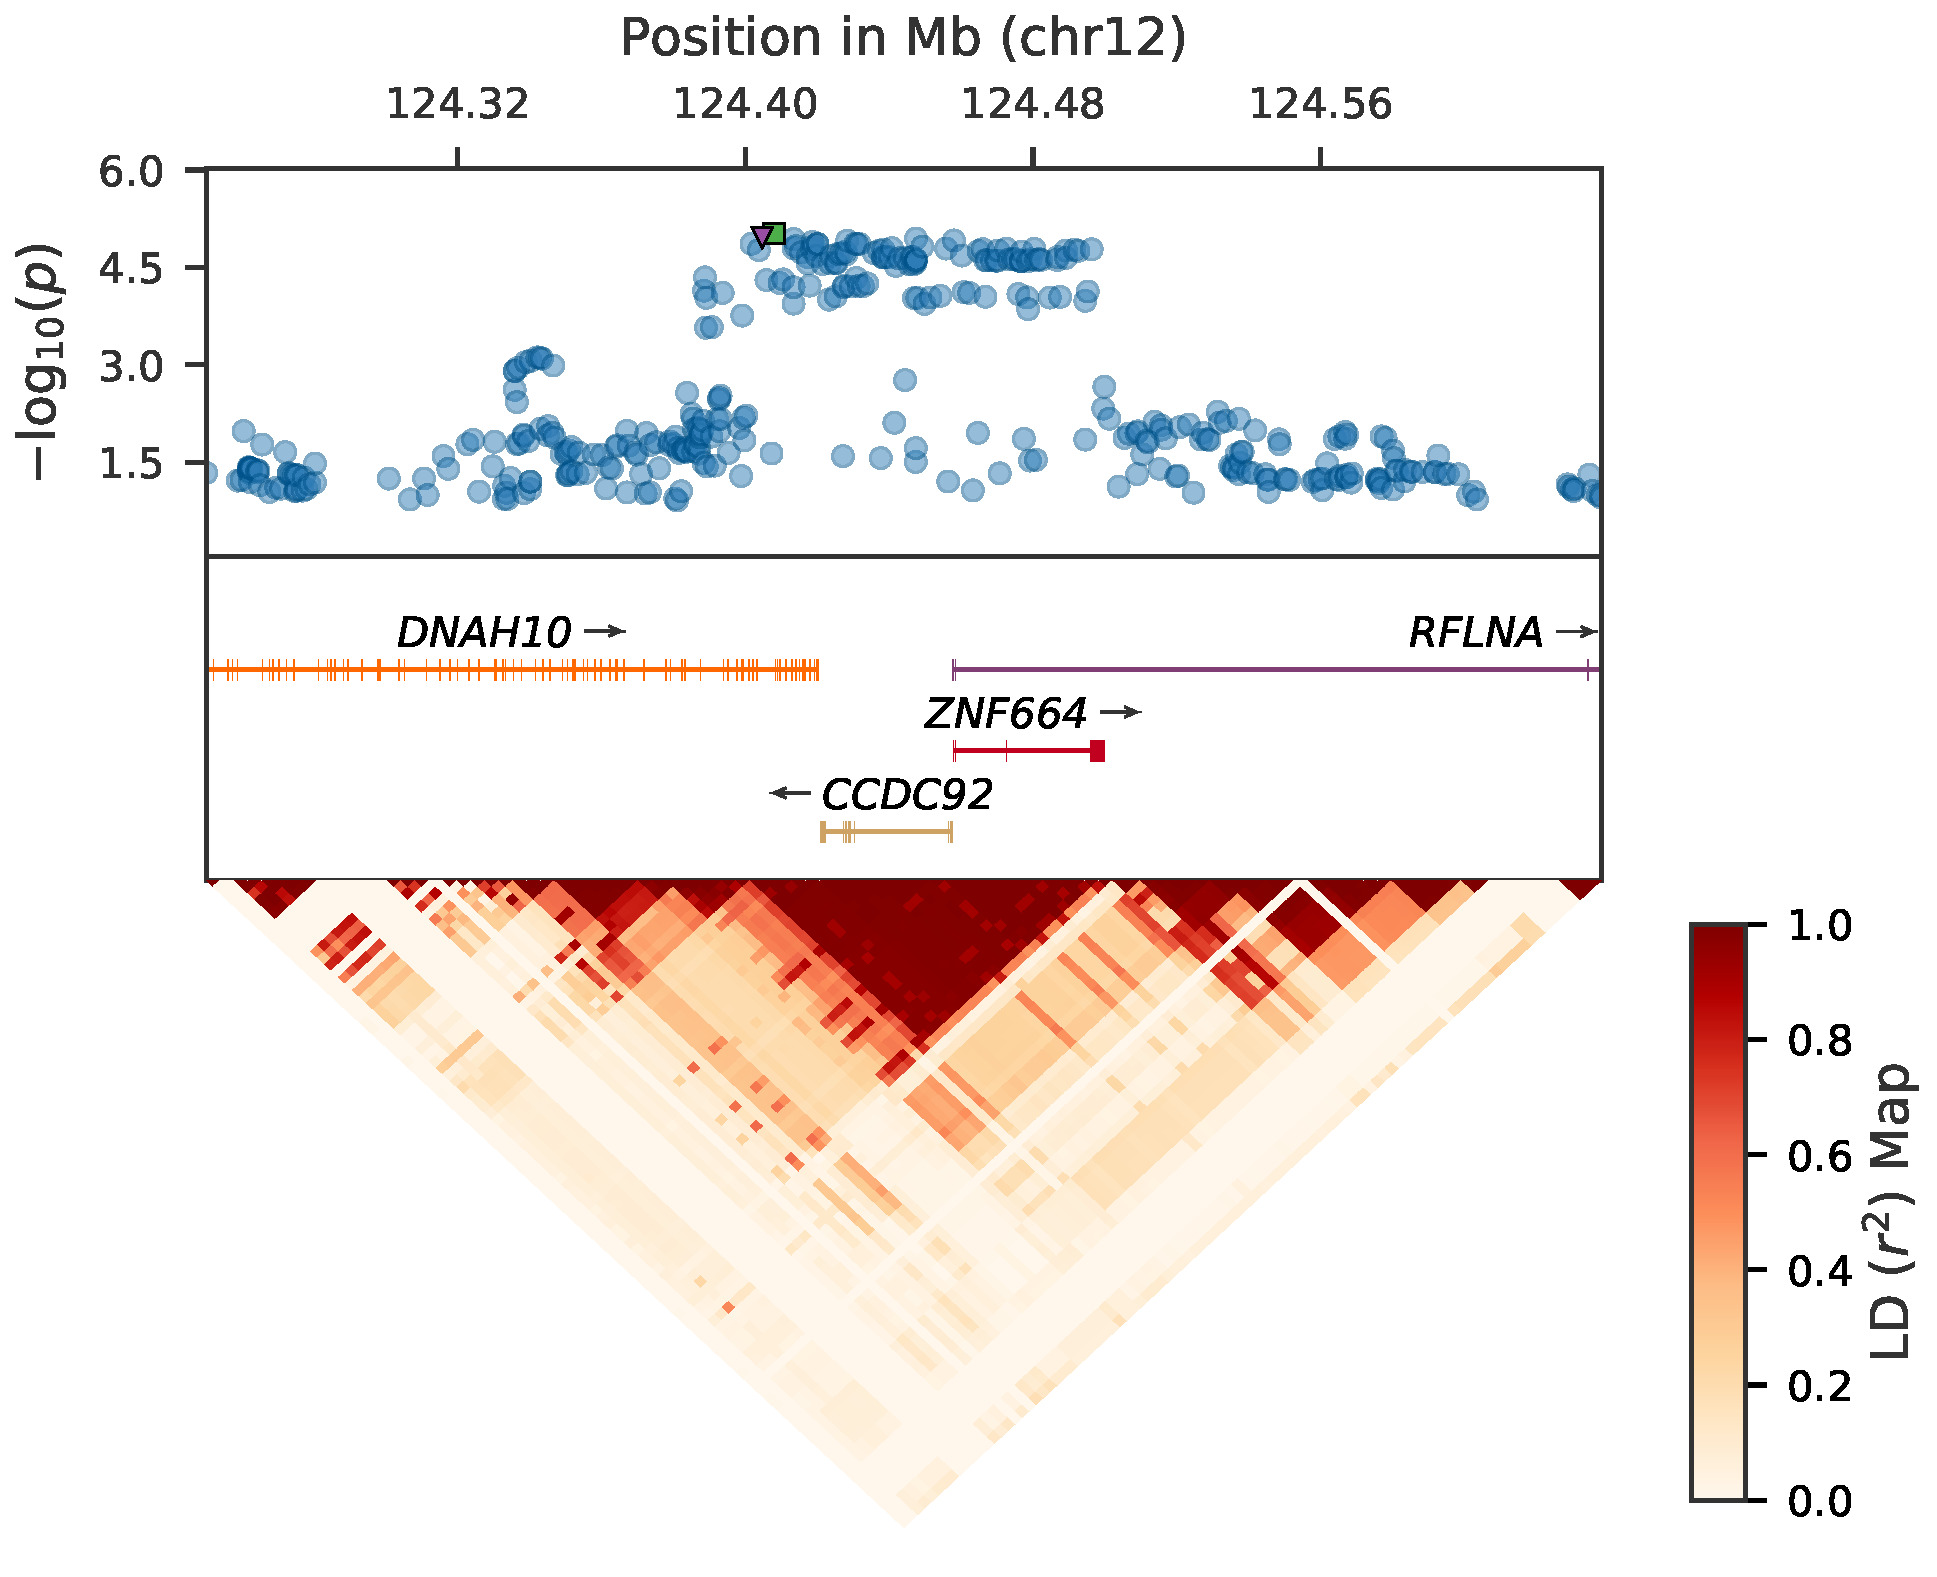
\includegraphics[height=15em]{Locus_013_ldexample.pdf}} & &
    \adjustbox{valign=m}{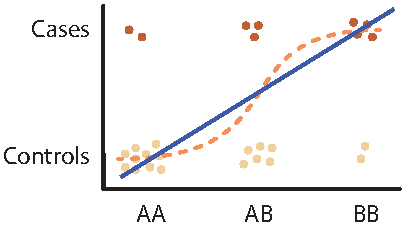
\includegraphics[height=10em]{linear_model.pdf}} \\[7.0em] 
    {\large Linkage disequilibrium \faFrownO} & & {\large Linear model \faFrownO} \\[0.5em]
  \end{tabular}
  } \\

  % Itemize on the right
  Multiple logistic regression should work much better in the non-linear regimes.\\
  {\textbf{Challenges for using multiple logistic regression}:}
  \begin{itemize}
    \item The integration for the maximum likelihood cannot be solved analytically.
    \item MCMC sampling is computationally intractable.
    \item Solutions using Laplace and linear approximations essentially makes it a linear model.
    \item Using multiple loci together for the analysis.
  \end{itemize} 
  \,\\[1.5em]
\end{multicols}

%\begin{tabular}{ccl}
%  { \specialcell{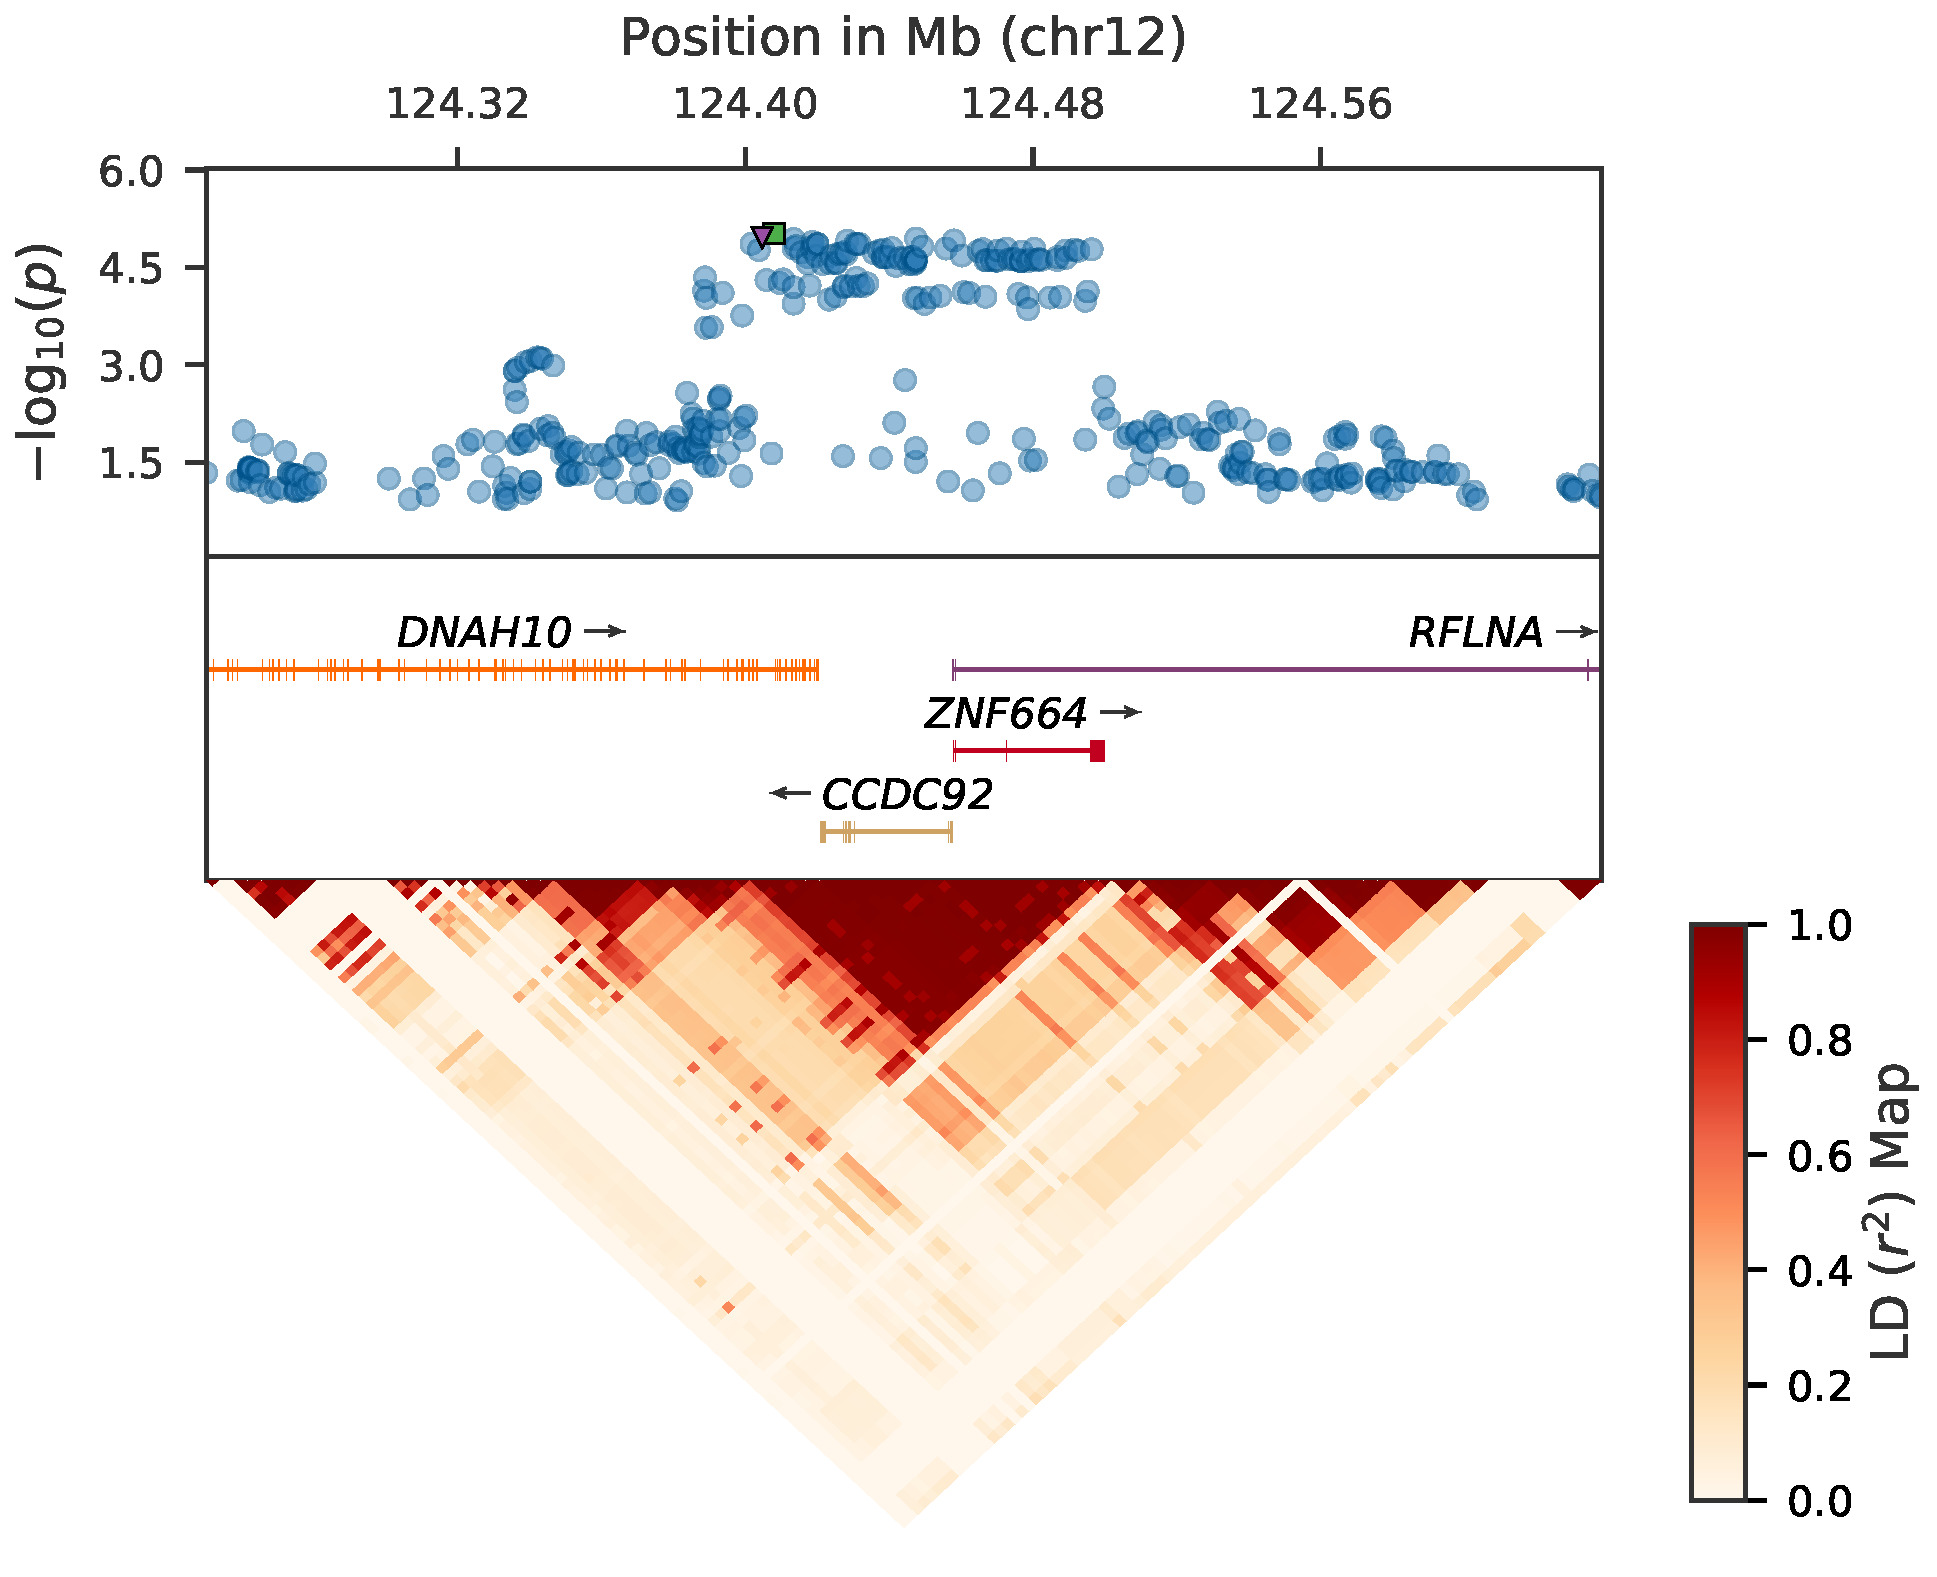
\includegraphics[height=15em]{Locus_013_ldexample.pdf} \\ Linkage disequilibrium \faFrownO} &
%  { \specialcell{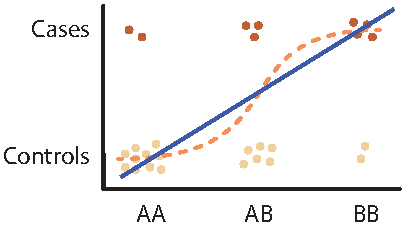
\includegraphics[height=15em]{linear_model.pdf} \\ Linear model \faFrownO} &
%  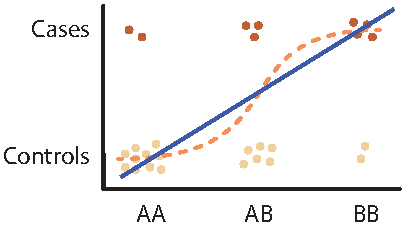
\includegraphics[width=10em]{linear_model.pdf}
%\end{tabular}


%\begin{tabular}{lll}
%  {\begin{center}
%    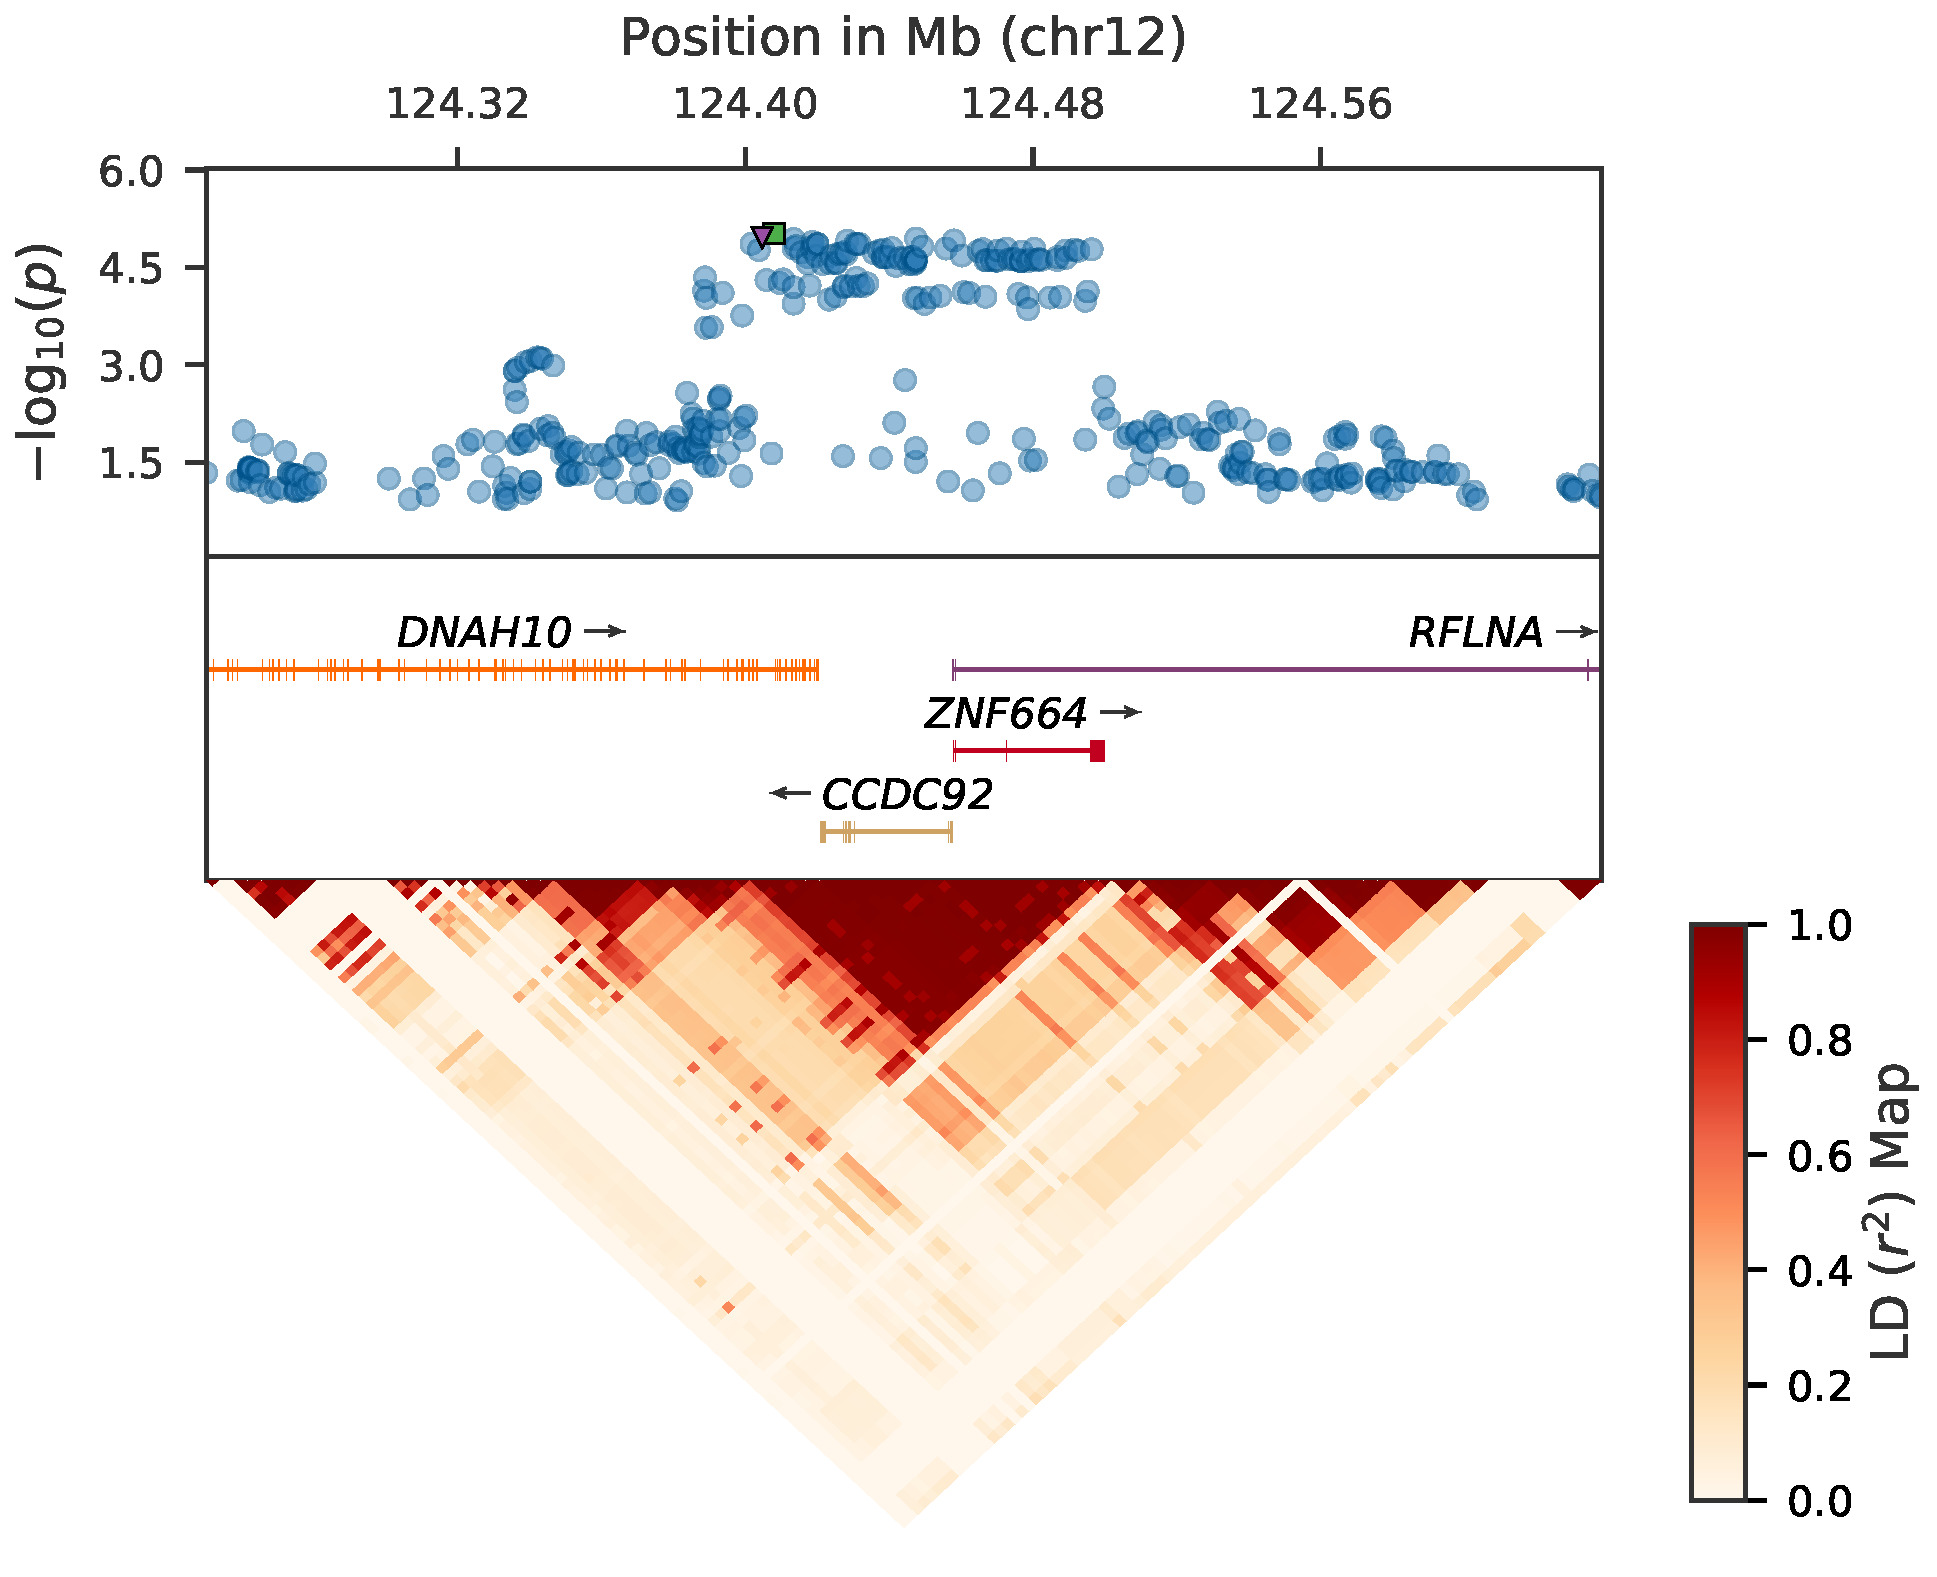
\includegraphics[width=0.2\textwidth]{Locus_013_ldexample.pdf} \\
%    Linkage disequilibrium \faFrownO \\
%  \end{center}
%  } &
%  {\begin{center}
%    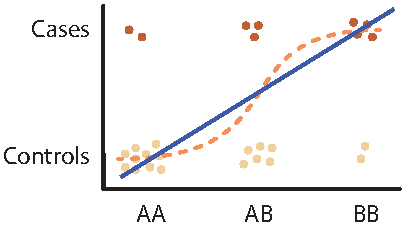
\includegraphics[width=0.3\textwidth]{linear_model.pdf}
%    Linear model \faFrownO \\
%  \end{center}
%  } &
%  {%{\large Challenges of multiple logistic regression:}
%    %\begin{itemize}
%    %  \item MCMC sampling is computationally intractable.
%    %  \item Laplace and linear approximations essentially makes it linear.
%    %\end{itemize}
%  } \\
%\end{tabular}

%\begin{multicols}{4}
%  {\begin{center}
%   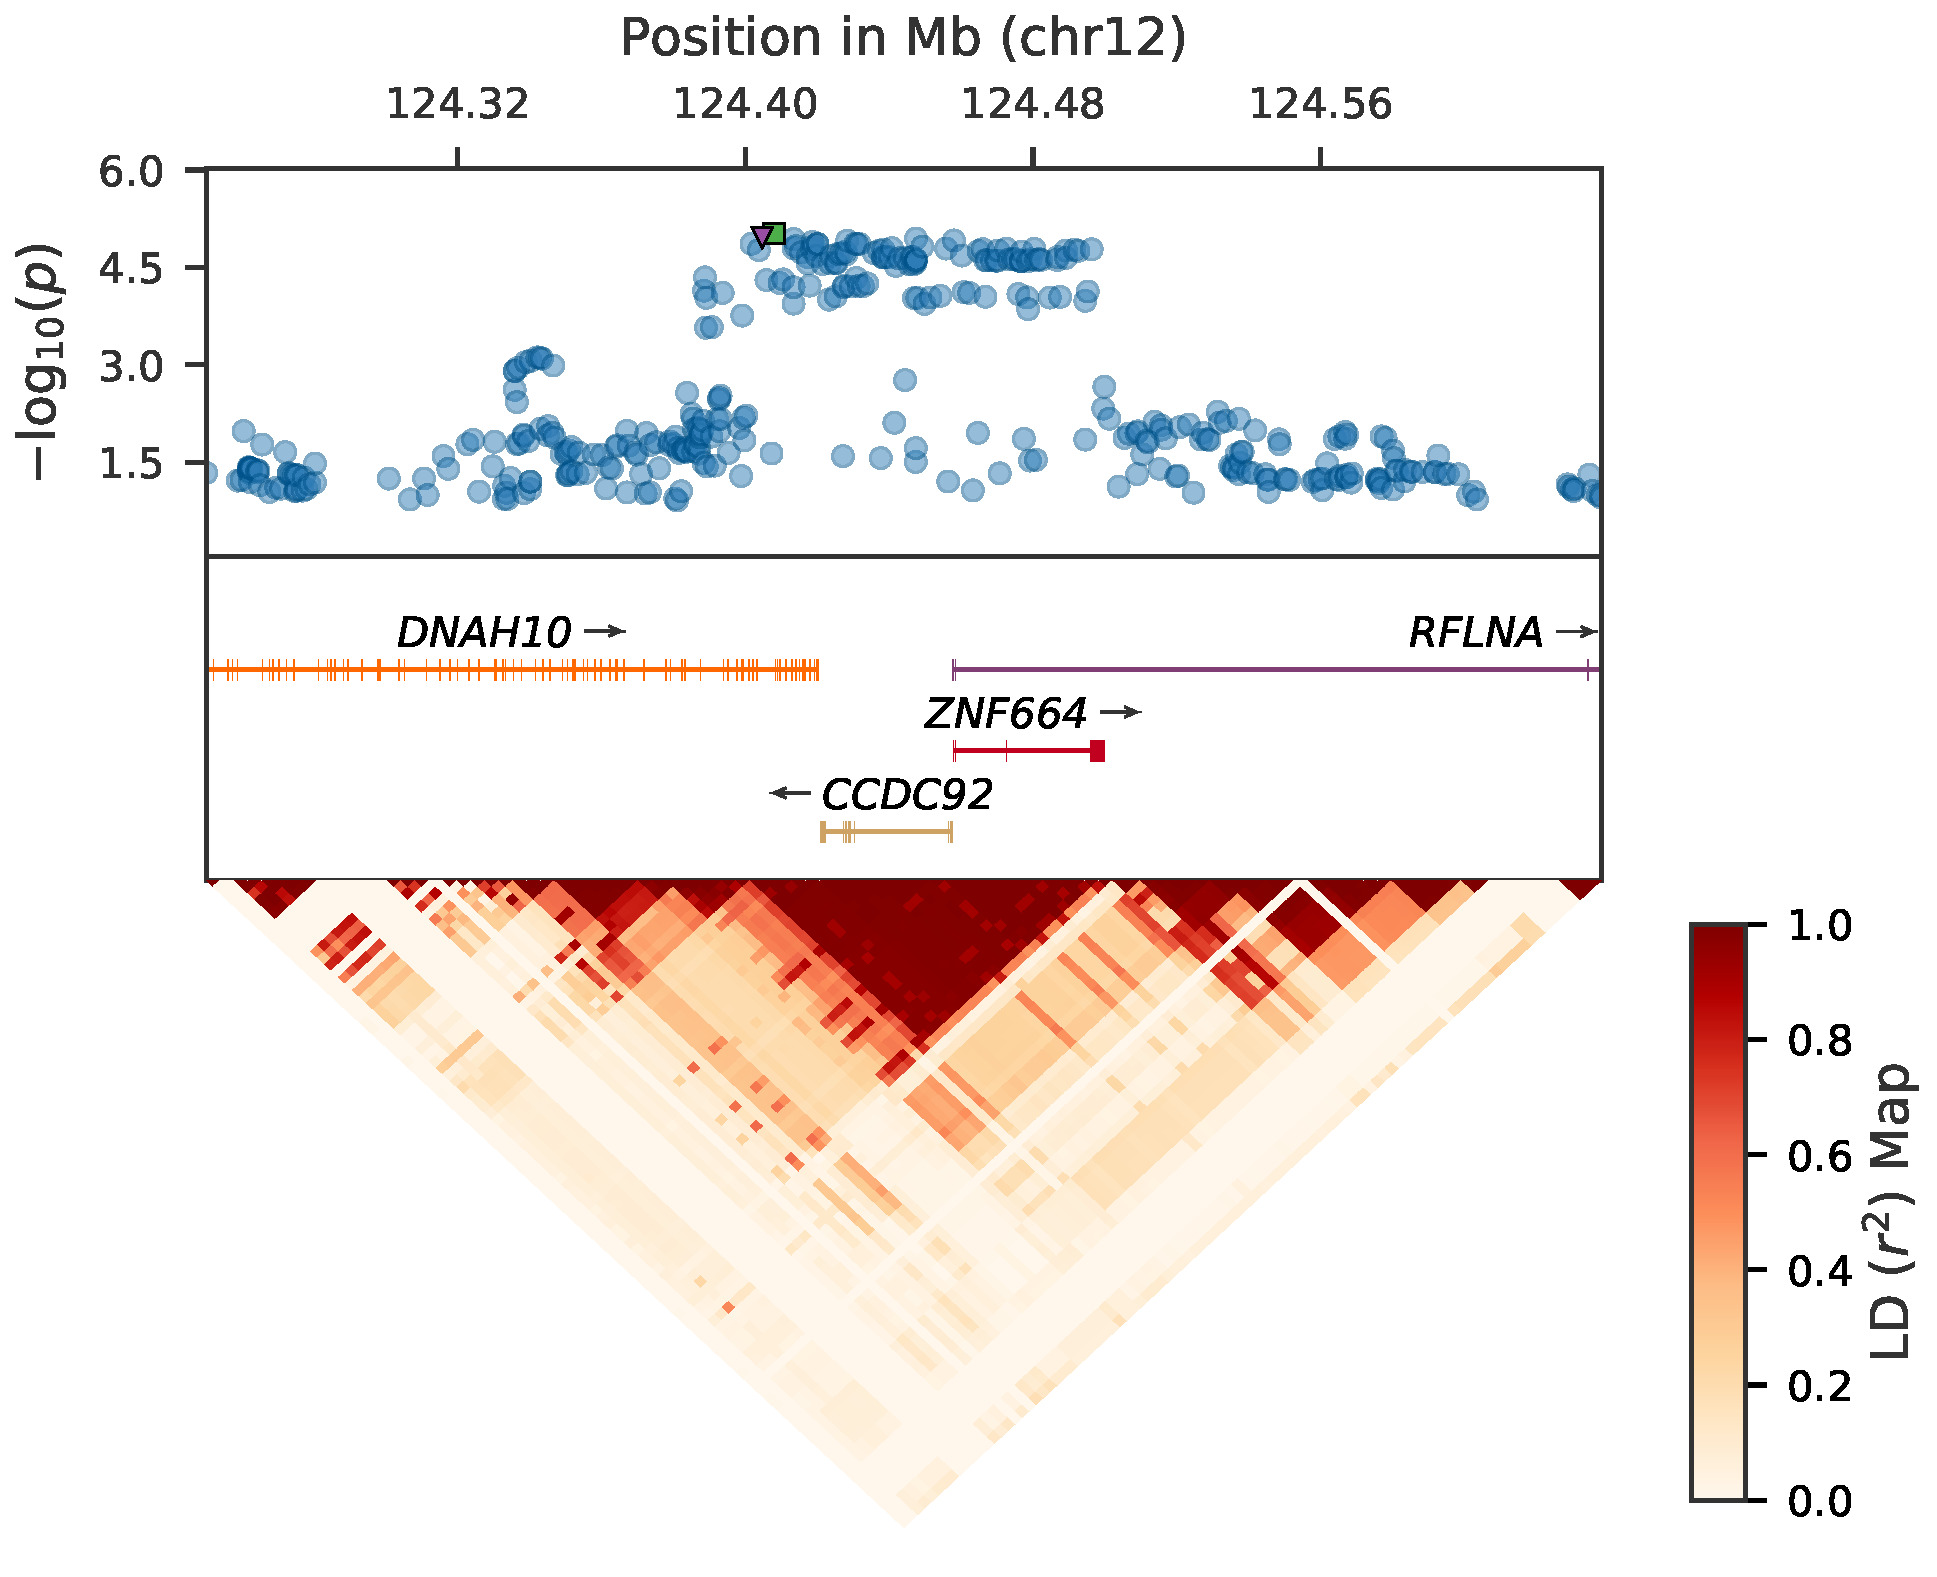
\includegraphics[width=0.2\textwidth]{Locus_013_ldexample.pdf} \\
%   Linkage disequilibrium \faFrownO \\
%   \end{center}
%  }
%  {\begin{center}
%   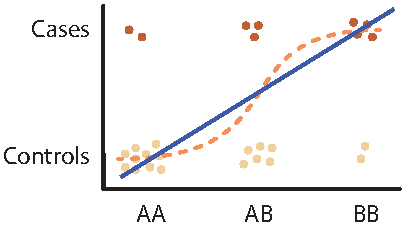
\includegraphics[width=0.3\textwidth]{linear_model.pdf}
%   Linear model \faFrownO \\
%   \end{center}
%  }
%  {\begin{center}
%   Multiple logistic regression 
%   \end{center}
%  }
%  {\begin{center}
%   How to solve the integral?
%   \end{center}
%  }
%\end{multicols}


  %{\begin{tikzpicture}
  %   \fill[fill = highlight!20] (0, 0) -- (7.5, 0) -- (8.5, 2.6) -- (7.5, 5.2) -- (0, 5.2) -- cycle;
  %   \node (simplereg) at (3.75, 2.6) [rectangle, align=justify, text width = 7cm, inner sep = 1em]
  %         {Genetic variants in genome-wide association studies (GWAS) are tested for disease association mostly using simple regression, one variant at a time.
  %          In post-GWAS analyses, such as finemapping, \textbf{\textsc{multiple regression}} use multiple SNPs with Bayesian variable selection,
  %          in which a sparsity-enforcing prior on effect sizes is used to avoid overtraining.
  %          The effect sizes are integrated out for posterior inference.};
  %          %For binary traits, the multiple \emph{logistic} regression has not yielded clear improvements over the linear model.};
  %   \fill[fill = mpibpcmaroon] (7.7, 0)    -- (22.5, 0.0) -- (23.1, 1.6) -- (8.3, 1.6)  -- cycle;
  %   \fill[fill = mpibpcblue] (8.35, 1.8) -- (23.15, 1.8) -- (23.5, 2.6) -- (23.15, 3.4) -- (8.35, 3.4) -- (8.7, 2.6) -- cycle;
  %   \fill[fill = mpibpcgreen] (8.3, 3.6)  -- (23.1, 3.6) -- (22.5, 5.2) -- (7.7, 5.2)  -- cycle;
  %   \node (improve1) at (15.5, 4.4) [rectangle, align=left, text width = 14cm, inner sep = 0em, color = black]
  %         {\textbf{\textsc{Multiple logistic regression}} has not yielded clear improvements over the linear model for binary traits in case-control GWAS.};
  %   \node (improve2) at (16.0, 2.6) [rectangle, align=left, text width = 14cm, inner sep = 0em, color = white]
  %         {\textbf{\textsc{MCMC sampling}} has proved to be costly and technically challenging to perform the integreation.};
  %   \node (improve3) at (15.5, 0.8) [rectangle, align=left, text width = 14cm, inner sep = 0em, color = white]
  %         {\textbf{\textsc{Linear approximation}} of the logistic function is often used for case-control data.};
  %   \fill [fill = important!20, inner sep = 0em] (23.7, 0) -- (29.5, 0) -- (29.5, 5.2) -- (23.7, 5.2) -- cycle;
  %   \node (blore) at (26.7, 2.6)%
  %         [rectangle, align=justify, text width = 5cm, inner sep = 0em]
  %         {\textbf{How to perform multiple logistic regression more accurately and faster?}
  %          \\[0.5em] In B-LORE, we introduce the \textbf{quasi-Laplace approximation} to analytically integrate over variant effect sizes. B-LORE improves finemapping with increasing number of controls.};
  % \end{tikzpicture}
  %}%
}

%%%%%%%%%%%%%%%%%%%%%
%%% METHODS %%%
%%%%%%%%%%%%%%%%%%%%%
\headerbox{2. B-LORE uses logistic model and sparsity-inducing priors}{name=model, column=0, row=1, span=2, below=motivation}{

  Probability of $n$\tss{th} individual with genotype $\vx_n$ to be diseased:
  \begin{multicols}{2}
    {\begin{center}
      \begin{tikzpicture}
        \node (a) at (0,0) [mathblock] {
          \begin{varwidth}{\linewidth}
          \begin{equation*}
            p\prth{\,y_n = 1 \mid \vx_n, \vv\,} = \frac{ \exp\prth{\,\vv^{\transpose}\vx_n} }{ 1 + \exp\prth{\,\vv^{\transpose}\vx_n} }
          \end{equation*}
          \end{varwidth}
        };
      \end{tikzpicture}
    \end{center}}
    {\begin{center} 
      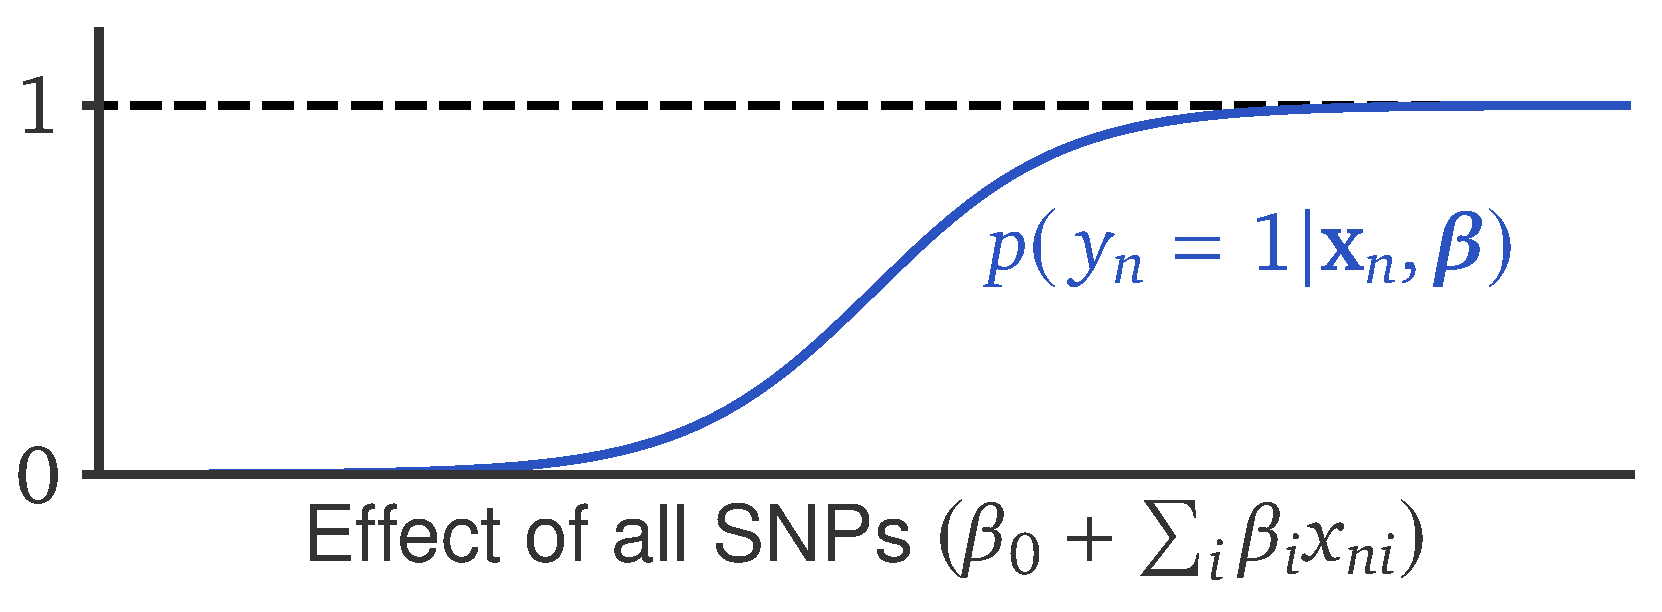
\includegraphics[width=0.4\textwidth]{logistic_function.pdf}
    \end{center}}
  \end{multicols}
  {\vspace{-2em}}%\color{primary}\noindent\rule{0.4\linewidth}{0.4pt}}\\[0.5em]
  Prior on effect sizes given hyperparameters $\pi$ and $\sigma$,
  {\vspace{-1em}}%\color{primary}\noindent\rule{0.4\linewidth}{0.4pt}}\\[0.5em]
  \begin{multicols}{2}
    {$\!
    \begin{aligned}
      & p\prth{\,\beta_i \mid \pi, \sigma} \nonumber\\ &=  
                                    {\color{secondary}\overbrace{\pi\,\N\prth{\beta_i \mid 0, \sigma^2}}^{\text{Causal}}} +
                                    {\color{primary}\overbrace{\prth{1 - \pi} \delta_0}^{\text{Non-causal}}} \nonumber \\[0.75em]
                                 &= \sum_{z_i = 0, 1} {\color{secondary} \pi^{z_i}} {\color{primary}\prth{1 - \pi}^{\prth{1 - z_i}}} 
                                    \N\prth{ \beta_i \mid \bf 0, \diag(\bs\sigma^2_{\vz, i}) } \nonumber \\
                                 &= \sum_{z_i = 0, 1} p\prth{ \vz \mid \pi } \N\prth{ \beta_i \mid \bf 0, \diag(\bs\sigma^2_{\vz, i}) } \nonumber \\
      \label{eq:effectsize-prior}
    \end{aligned}
    $\\[-0.5em]
    where, $\sigma^2_{\vz,i} = z_i \sigma^2 $ \\[0.5em]
    $z_i \in \{0, 1\} \Rightarrow$ Indicator variable of causality \\[0.5em]
    }%
    {\begin{center}
      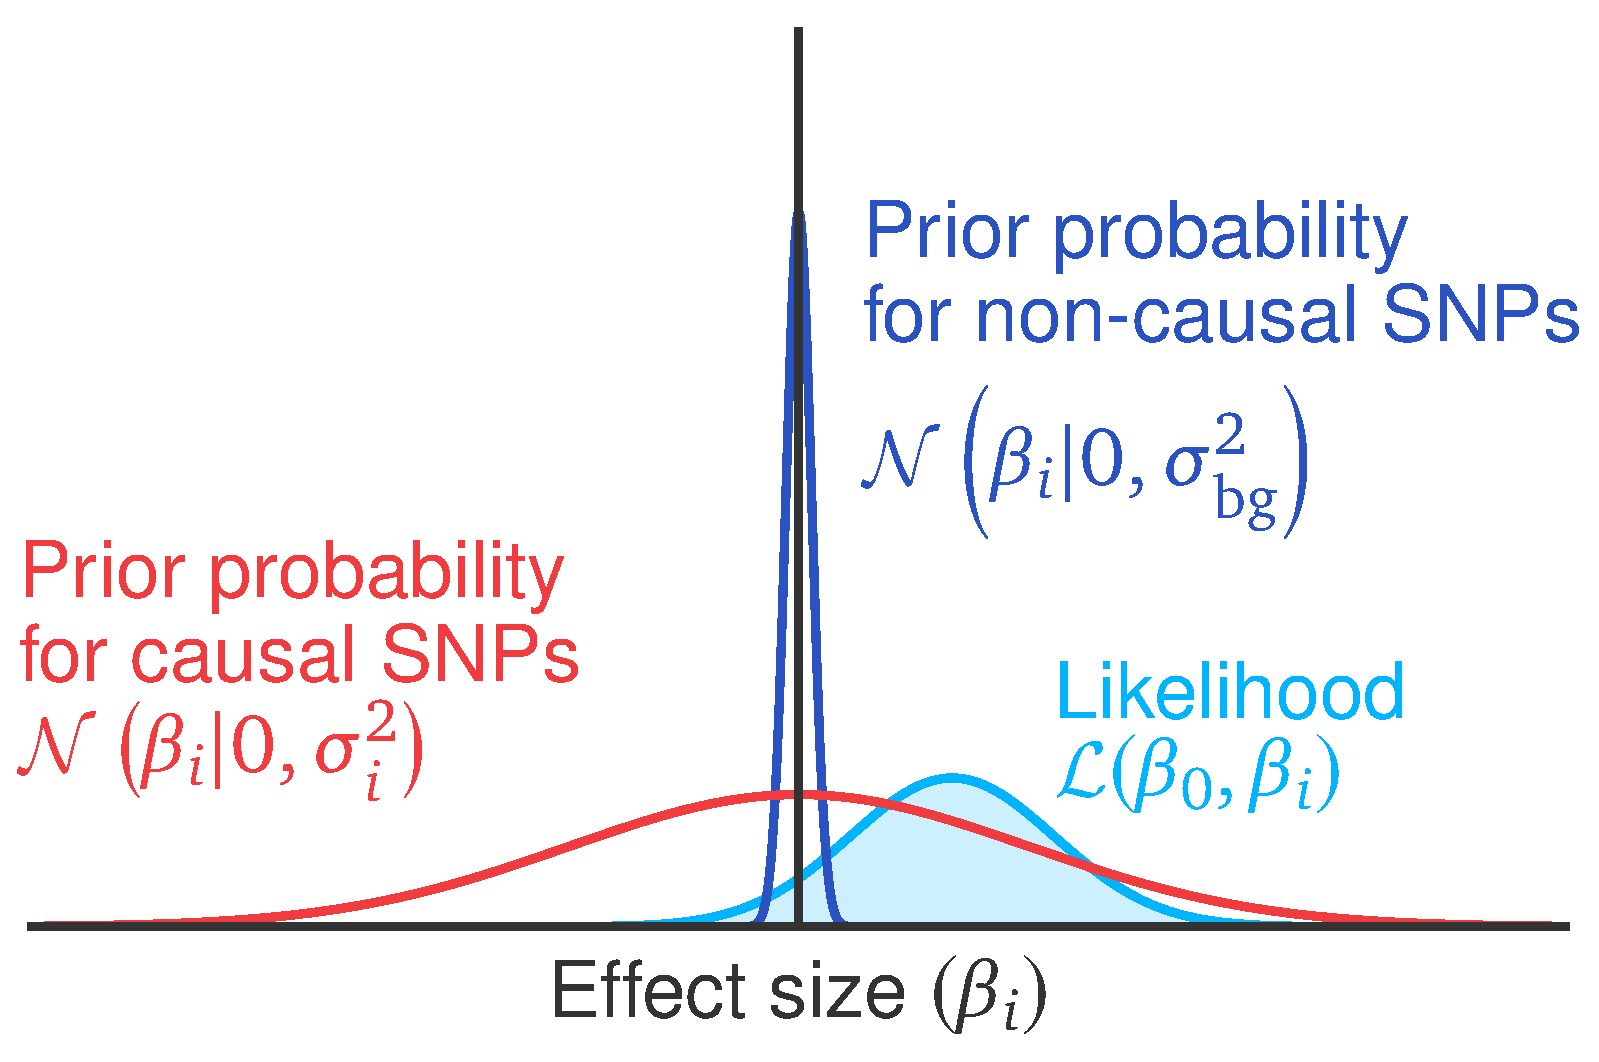
\includegraphics[width=0.43\textwidth]{bayesian_logistic_regression.pdf} \\
      \begin{tikzpicture}
        \node (a) at (0,0) [infoblock] {
            \begin{varwidth}{\linewidth}
            \begin{itemize}[leftmargin=1.2em, label={\color{primary}\tiny\DiamondSolid}]
              \setlength\itemsep{0.1em}
              \item $z_i = 1$ \qquad SNP $i$ is causal
              \item $z_i = 0$ \qquad SNP $i$ is non-causal
            \end{itemize}
            \end{varwidth}
        };
      \end{tikzpicture}
    \end{center}}
  \end{multicols}
}

\headerbox{3. We introduce the quasi-Laplace approximation}{name=optim, column=2, span=2, below=motivation, bottomaligned=model}{

  \emph{Evidence approximation}: maximizing the marginal likelihood\\[-0.5em]
  \begin{equation*}
    \mathrm{m}\mathcal{L}(\pi, \sigma) := p \prth{ \vy \mid \vx, \pi, \sigma }
                    = \sum_{\vz} {\color{black} p\prth{ \vz \mid \pi }}
                      \int {\color{sub2} p \prth{ \vy \mid \vx, \vv }}\,
                           {\color{sub1} \mathcal{N}\prth{ \vv \mid \bf 0, \diag\prth{\bs\sigma^2_\vz} }} d\vv \rightarrow \max
  \end{equation*}

  \vspace{0.75em}
  {\textbf{Quasi-Laplace approximation}:}
  \begin{equation*}
    {\color{sub2} p\prth{ \vy \mid \vx, \vv }}\, {\color{sub1} \mathcal{N}\prth{ \vv \mid \bf 0, \diag\prth{\bs\sigma^2_\vz} }} =
       {\color{black} \underbrace{ {\color{sub2} p\prth{ \vy \mid \vx, \vv }}\, {\color{black} \mathcal{N}\prth{\vv \mid \bf 0,\: \tilde{\sigma}^2\identity }} }_{
                       \displaystyle \propto \mathcal{N} \prth{ \vv \mid \tilde{\vv}, \tilde{\bs\Lambda}^{-1} }}
       }
      \frac{{\color{sub1}\mathcal{N}\prth{ \vv \mid \bf 0, \diag\prth{\bs\sigma^2_\vz} }}}{\color{black} \mathcal{N}\prth{\vv \mid \bf 0,\: \tilde{\sigma}^2\identity }}
  \end{equation*}

  {\textbf{Benefits}:}
  \begin{itemize}
    \item The regularizer pulls the maximum of the regularized likelihood near to the mode of the integral, making it more accurate than Laplace approximation.
    \item Can be extended to multiple studies.
    \item Fast gradient-descent optimization.
  \end{itemize}
  {\begin{center}
    \begin{tikzpicture}
      \fill[fill = highlight!20] (0, 0) -- (2.5, 0) -- (3, 0.9) -- (2.5, 1.8) -- (0, 1.8) -- cycle;
      \fill[fill = mpibpcmaroon] (2.7, 0) -- (14, 0) -- (14, 0.8) -- (3.15, 0.8) -- cycle;
      \fill[fill = mpibpcblue]   (3.15, 1) -- (14, 1) -- (14, 1.8) -- (2.7, 1.8) -- cycle;
      %\fill[fill = mpibpcmaroon!80] (5, 0) -- (14, 0) -- (14, 0.8) -- (5, 0.8) -- cycle;
      %\fill[fill = mpibpcblue!80]   (5, 1) -- (14, 1) -- (14, 1.8) -- (5, 1.8) -- cycle;
      \node at (1.25, 0.9) [rectangle, align=center, text width = 2cm, inner sep = 0em, color=black] {\textbf{B-LORE} schema};
      \node at (8.5, 1.4) [rectangle, align=center, inner sep = 0em, color=white]
                          {1. Two-step optimization at each cohort to estimate $\tilde{\sigma}$ and ($\tilde{\vv}, \tilde{\bs\Lambda}$).};
      \node at (8.5, 0.4) [rectangle, align=justify, inner sep = 0em, color=white]
                          {2. Estimation of hyperparameters ($\pi$, $\sigma$).%
%                              by optimizing the marginal likelihood using $\tilde{\sigma}$, $\tilde{\vv}$ and $\tilde{\bs\Lambda}$ of each study.
                          };
    \end{tikzpicture}
  \end{center}}
}

\headerbox{4. Inference}{name=infer, column=3, span=1, below=optim}{
  {\color{primary}\emph{Prediction of causality of each locus}.}\\[0.5em]
  The probability for a locus to be causally associated with the disease is%= 1 -- probability of {\scshape not} containing a single causal SNP.
  {\begin{center} \vskip-1.5em
    \begin{tikzpicture}
      \node (a) at (0,0) [highlightnosep] {
          \begin{varwidth}{\linewidth}
            \begin{align*}
              \prob_{\mathrm{causal}} &= p\prth{\text{locus is causal} \mid \bs\phi, \vX, \hat\pi, \hat\sigma} \\
                                      &= 1 - p\prth{\vz = 0 \mid \bs\phi, \vX, \hat\pi, \hat\sigma}
            \end{align*}
          \end{varwidth}
      };
    \end{tikzpicture}
  \end{center}}

  {\color{primary}\emph{Statistical finemapping of causal variants}.}\\[0.5em]
  The posterior probability for SNP $i$ to be causal is 
  {\begin{center} \vskip-0.5em
    \begin{tikzpicture}
      \node (a) at (0,0) [highlight] {
          \begin{varwidth}{\linewidth}
            \begin{equation*}
              p\prth{z_i = 1 \mid \bs\phi, \vX, \hat\pi, \hat\sigma}
            \end{equation*}
          \end{varwidth}
      };
    \end{tikzpicture}
  \end{center}}
}

%%%%%%%%%%%%%%%%%%%%%%%%%%%%%%%%%%%
%%%% GERMIFS CAD %%%
%%%%%%%%%%%%%%%%%%%%%%%%%%%%%%%%%%%
\headerbox{5. Meta-analysis example: B-LORE discovers novel loci associated with coronary artery disease}{name=realcad, column=0, span=3, below=model}{
\newdimen\myfigheight
\setlength{\myfigheight}{8cm}

  \begin{center}
    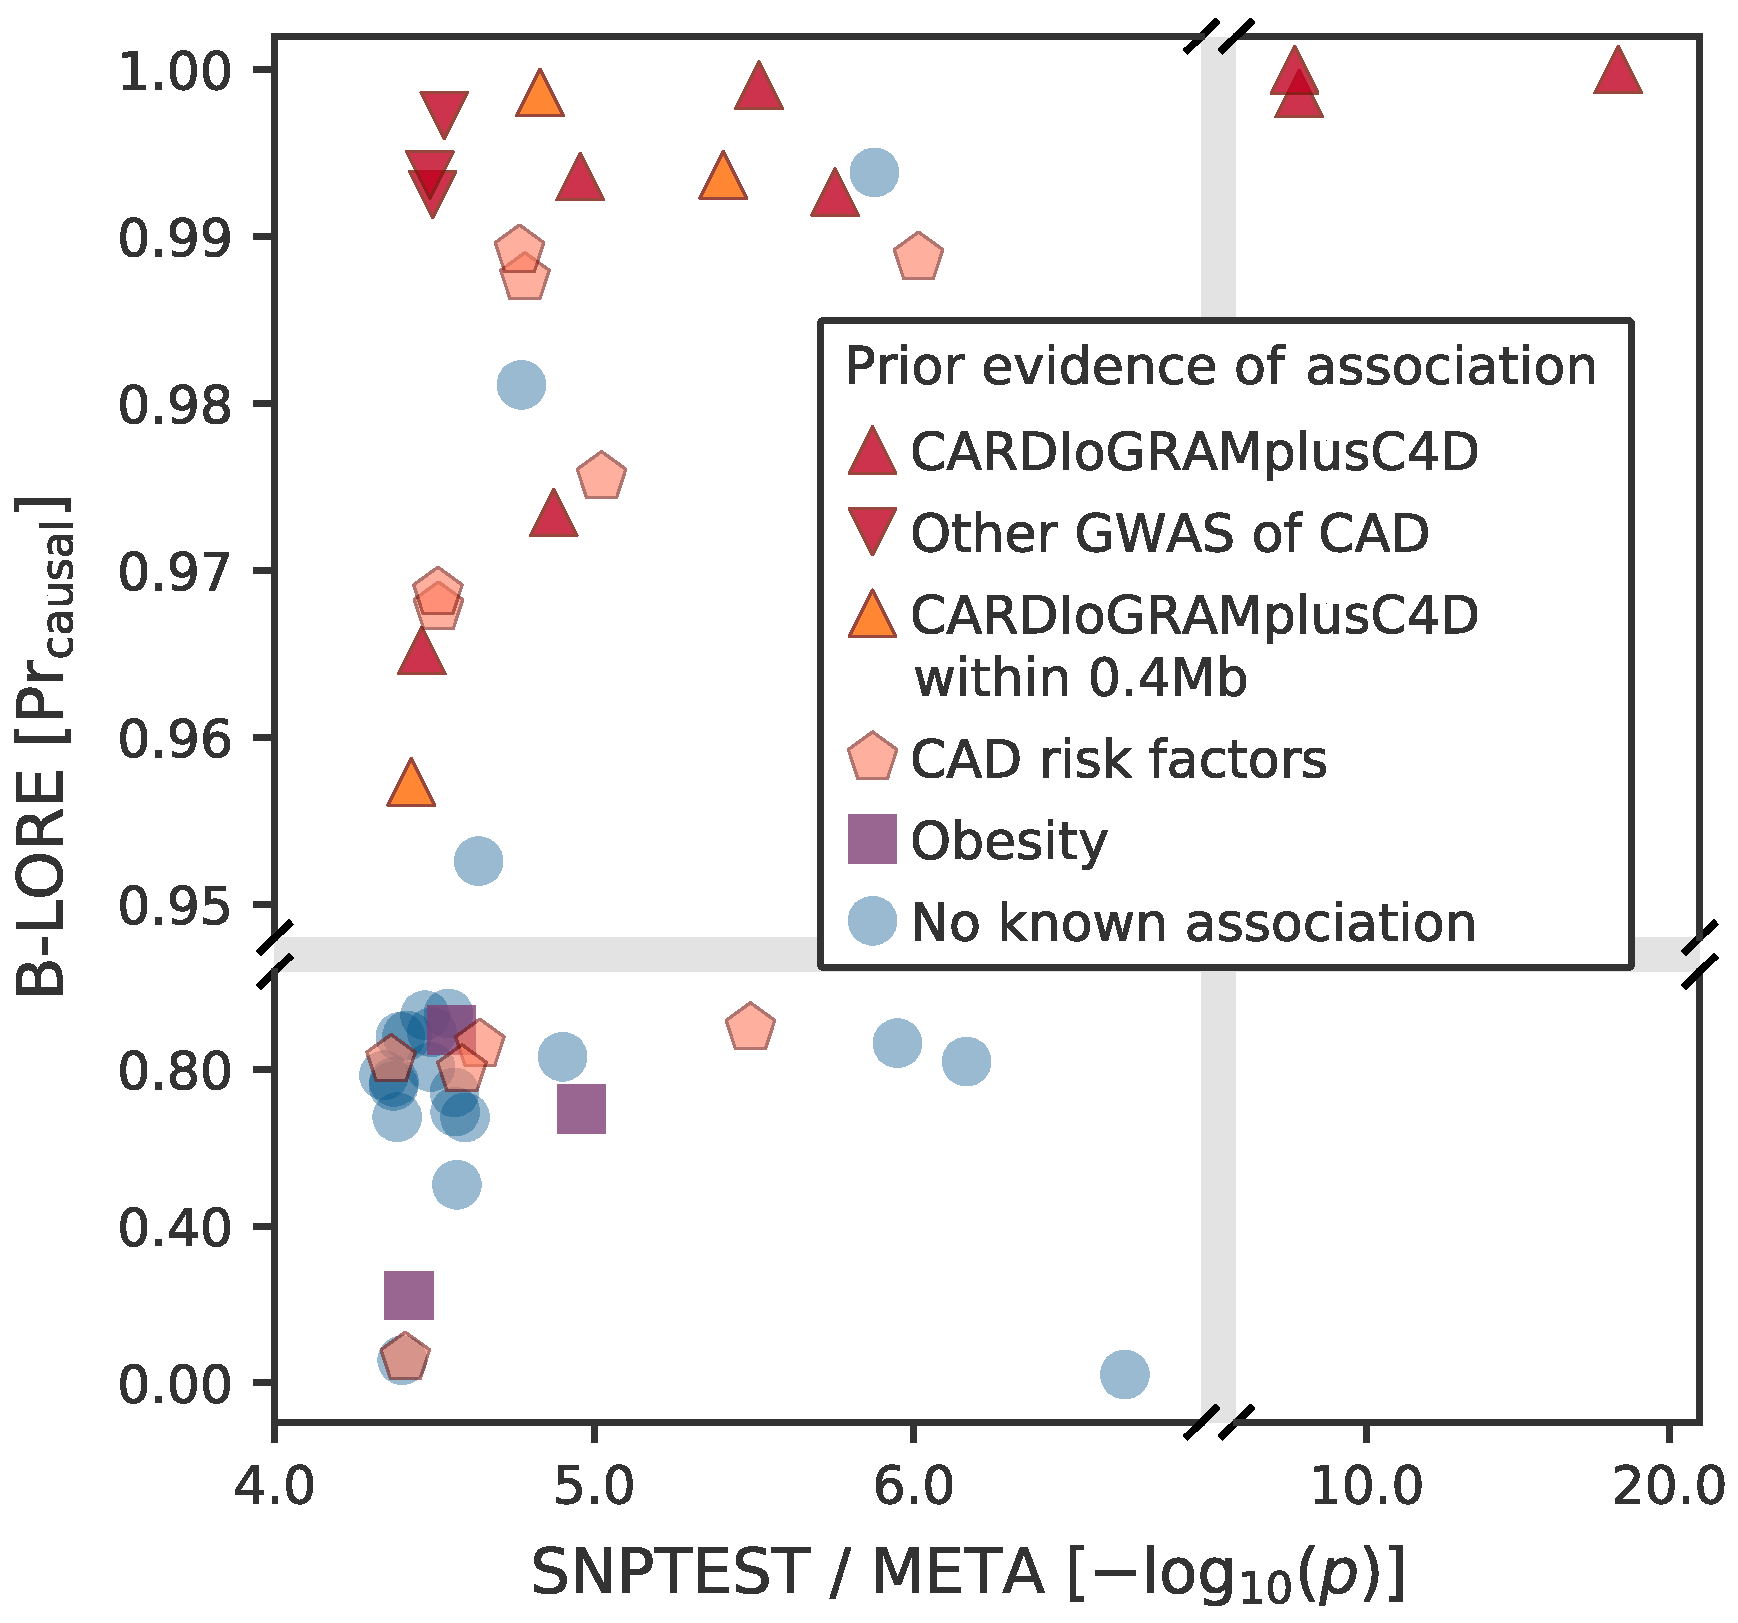
\includegraphics[height=\myfigheight, keepaspectratio]{loci_classification.pdf}
    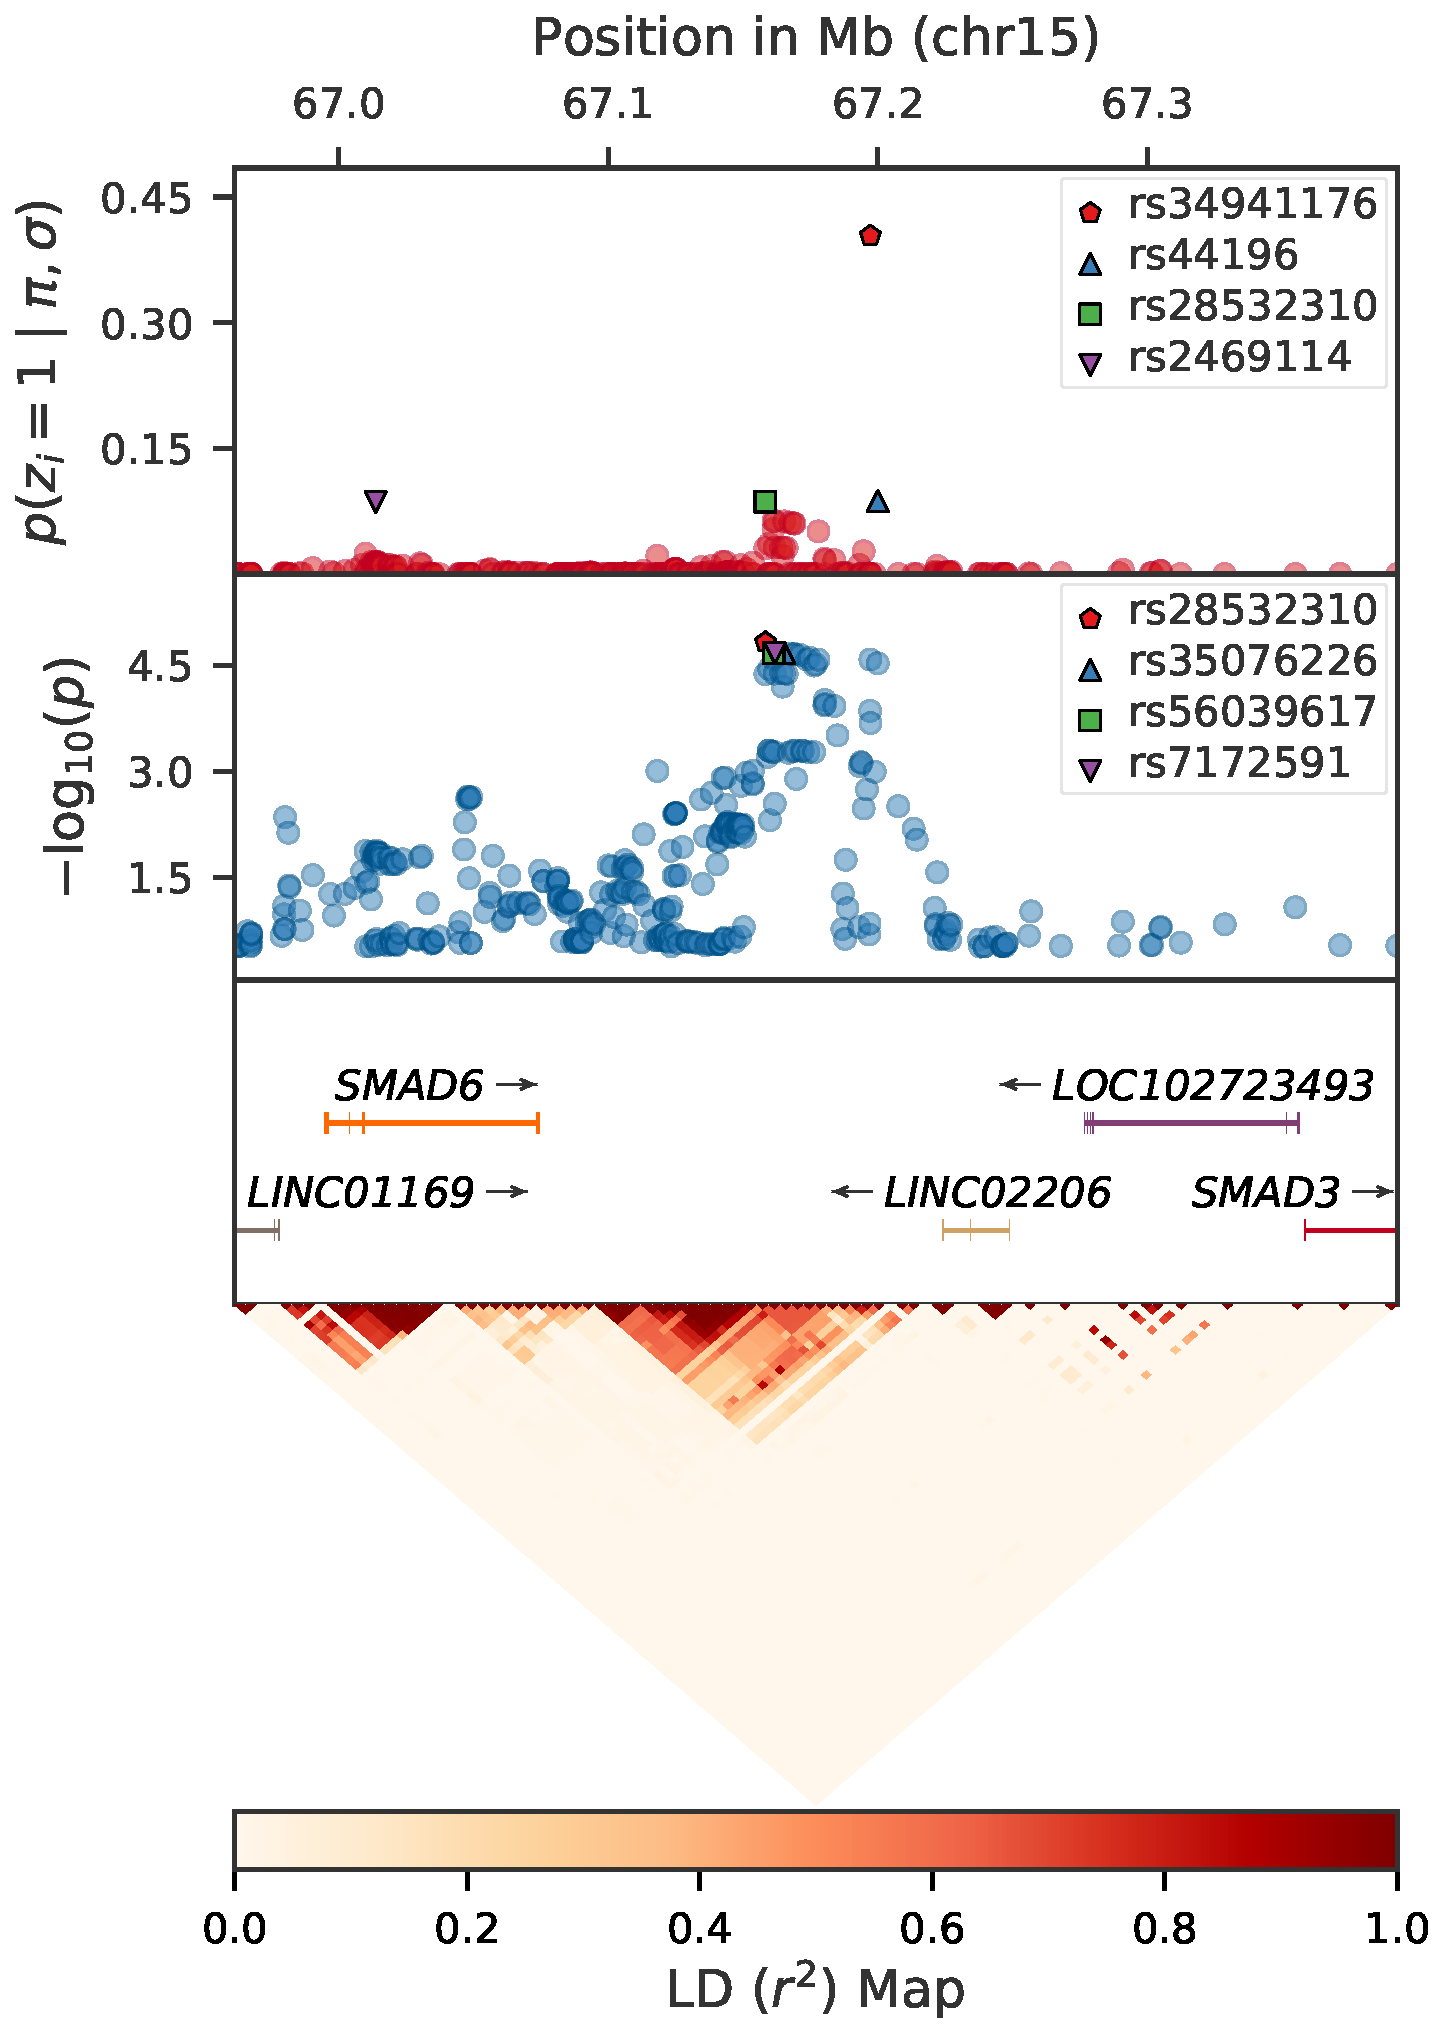
\includegraphics[height=\myfigheight, keepaspectratio]{Locus_018.pdf}
    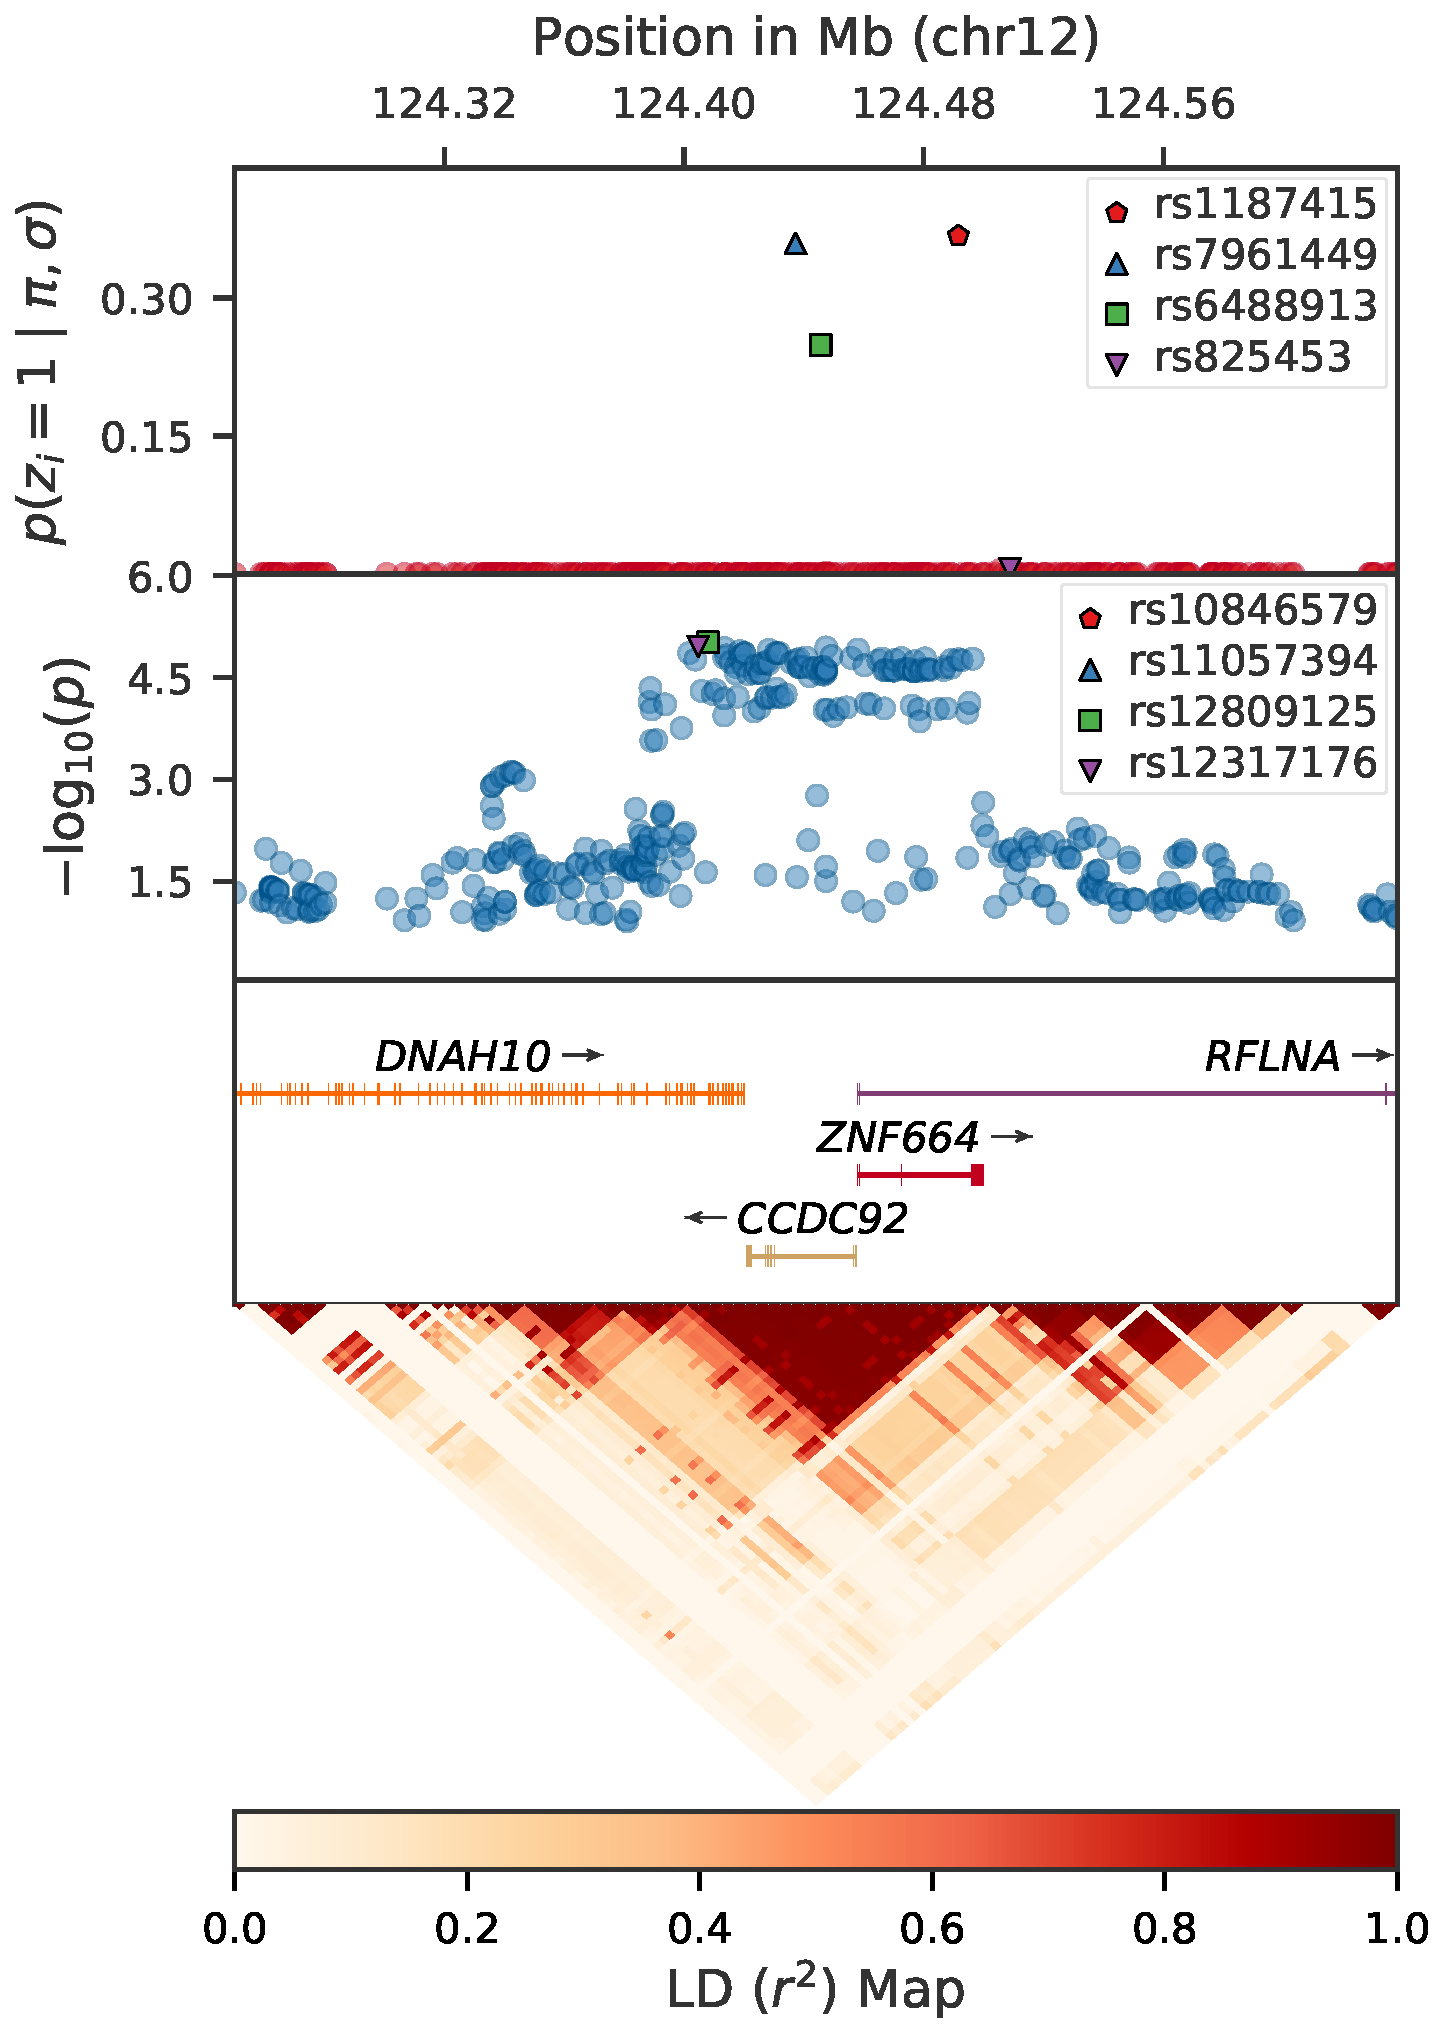
\includegraphics[height=\myfigheight, keepaspectratio]{Locus_013.pdf}
  \end{center}
Meta-analysis of 5 cohorts, Germal Myocardial Infarction Family Studies (GerMIFS I-V) -- 6234 cases and 6848 controls.
%Meta-analysis of 5 cohorts (Germal Myocardial Infarction Family Study, GerMIFS I-V) with a total of 6234 cases and 6848 controls from white European ancestry. 
%We pre-selected the top 50 loci with SNPTEST / META, and applied B-LORE.
}


%%%%%%%%%%%%%%%%%%%%%%%%%%%%%%%%%%e
%%%% SIMULATION RESULTS %%%
%%%%%%%%%%%%%%%%%%%%%%%%%%%%%%%%%%%
\headerbox{6. Examples of non-linear regimes in case-control GWAS}{name=simures, column=0, span=3, below=realcad}{

  %{We simulated 13082 phenotypes for 5 cohorts usings 100 loci of $\sim$200 SNPs, using one or more causal SNPs in each locus.}

\begin{multicols}{4}
  {\begin{center}
   $h_g^2 = 0.4$\\
   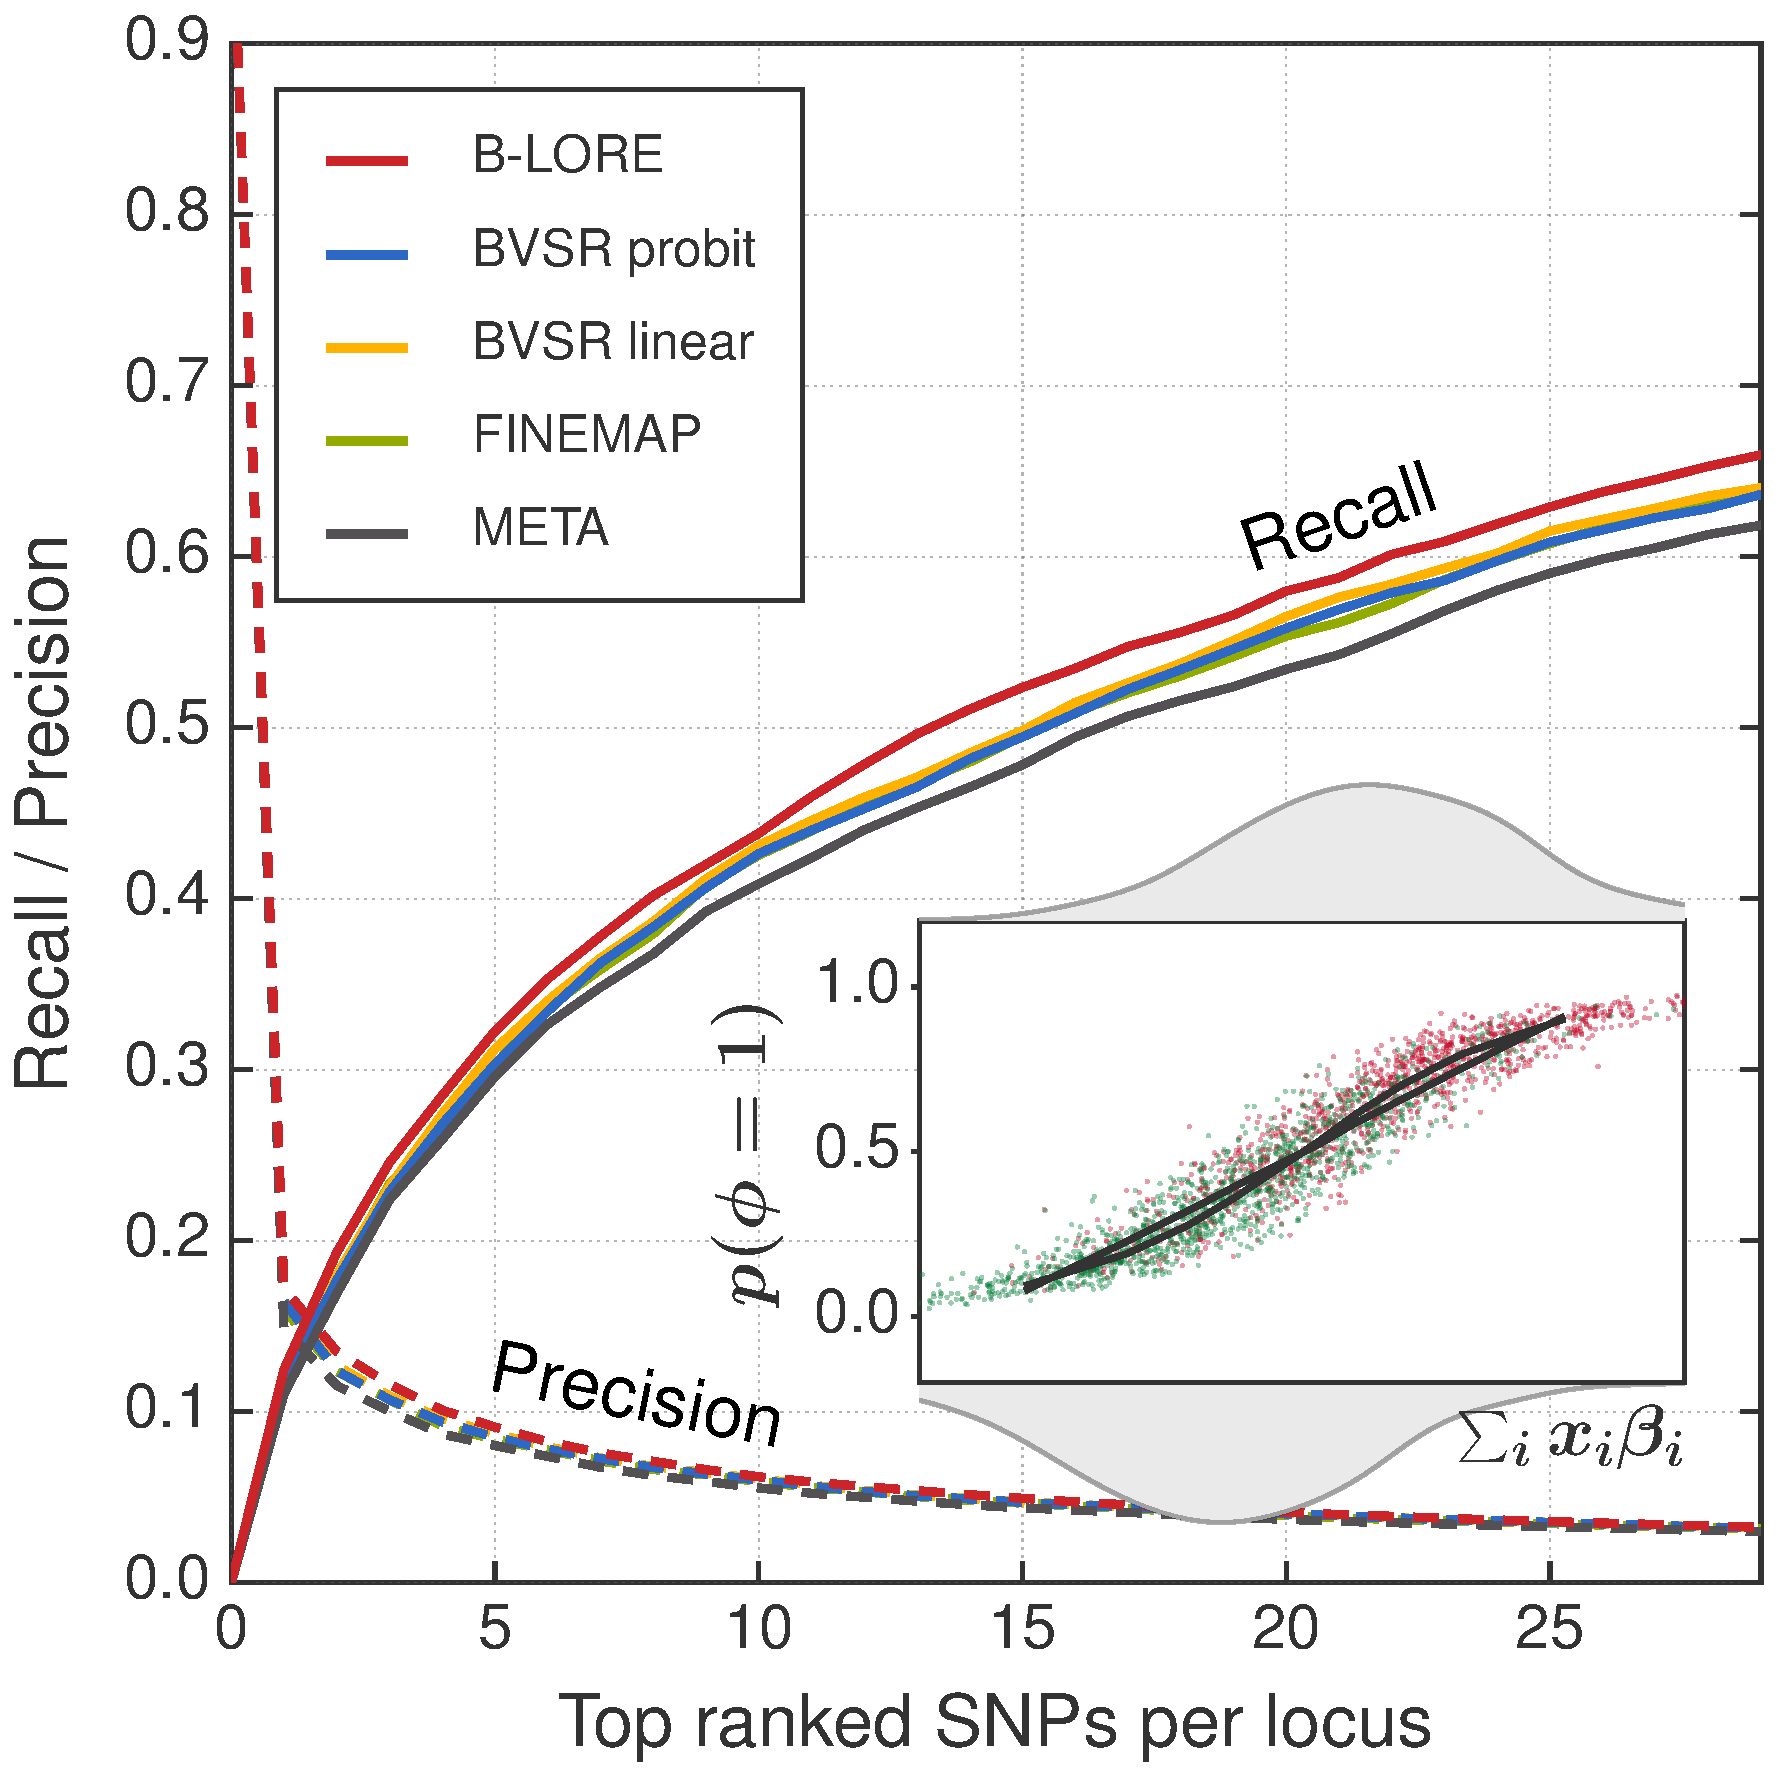
\includegraphics[width=0.23\textwidth]{pip_prc_normal_h04_c2_l100_cred.pdf}
   \end{center}
  }
  {\begin{center}
   $h_g^2 = 0.8$ \\
   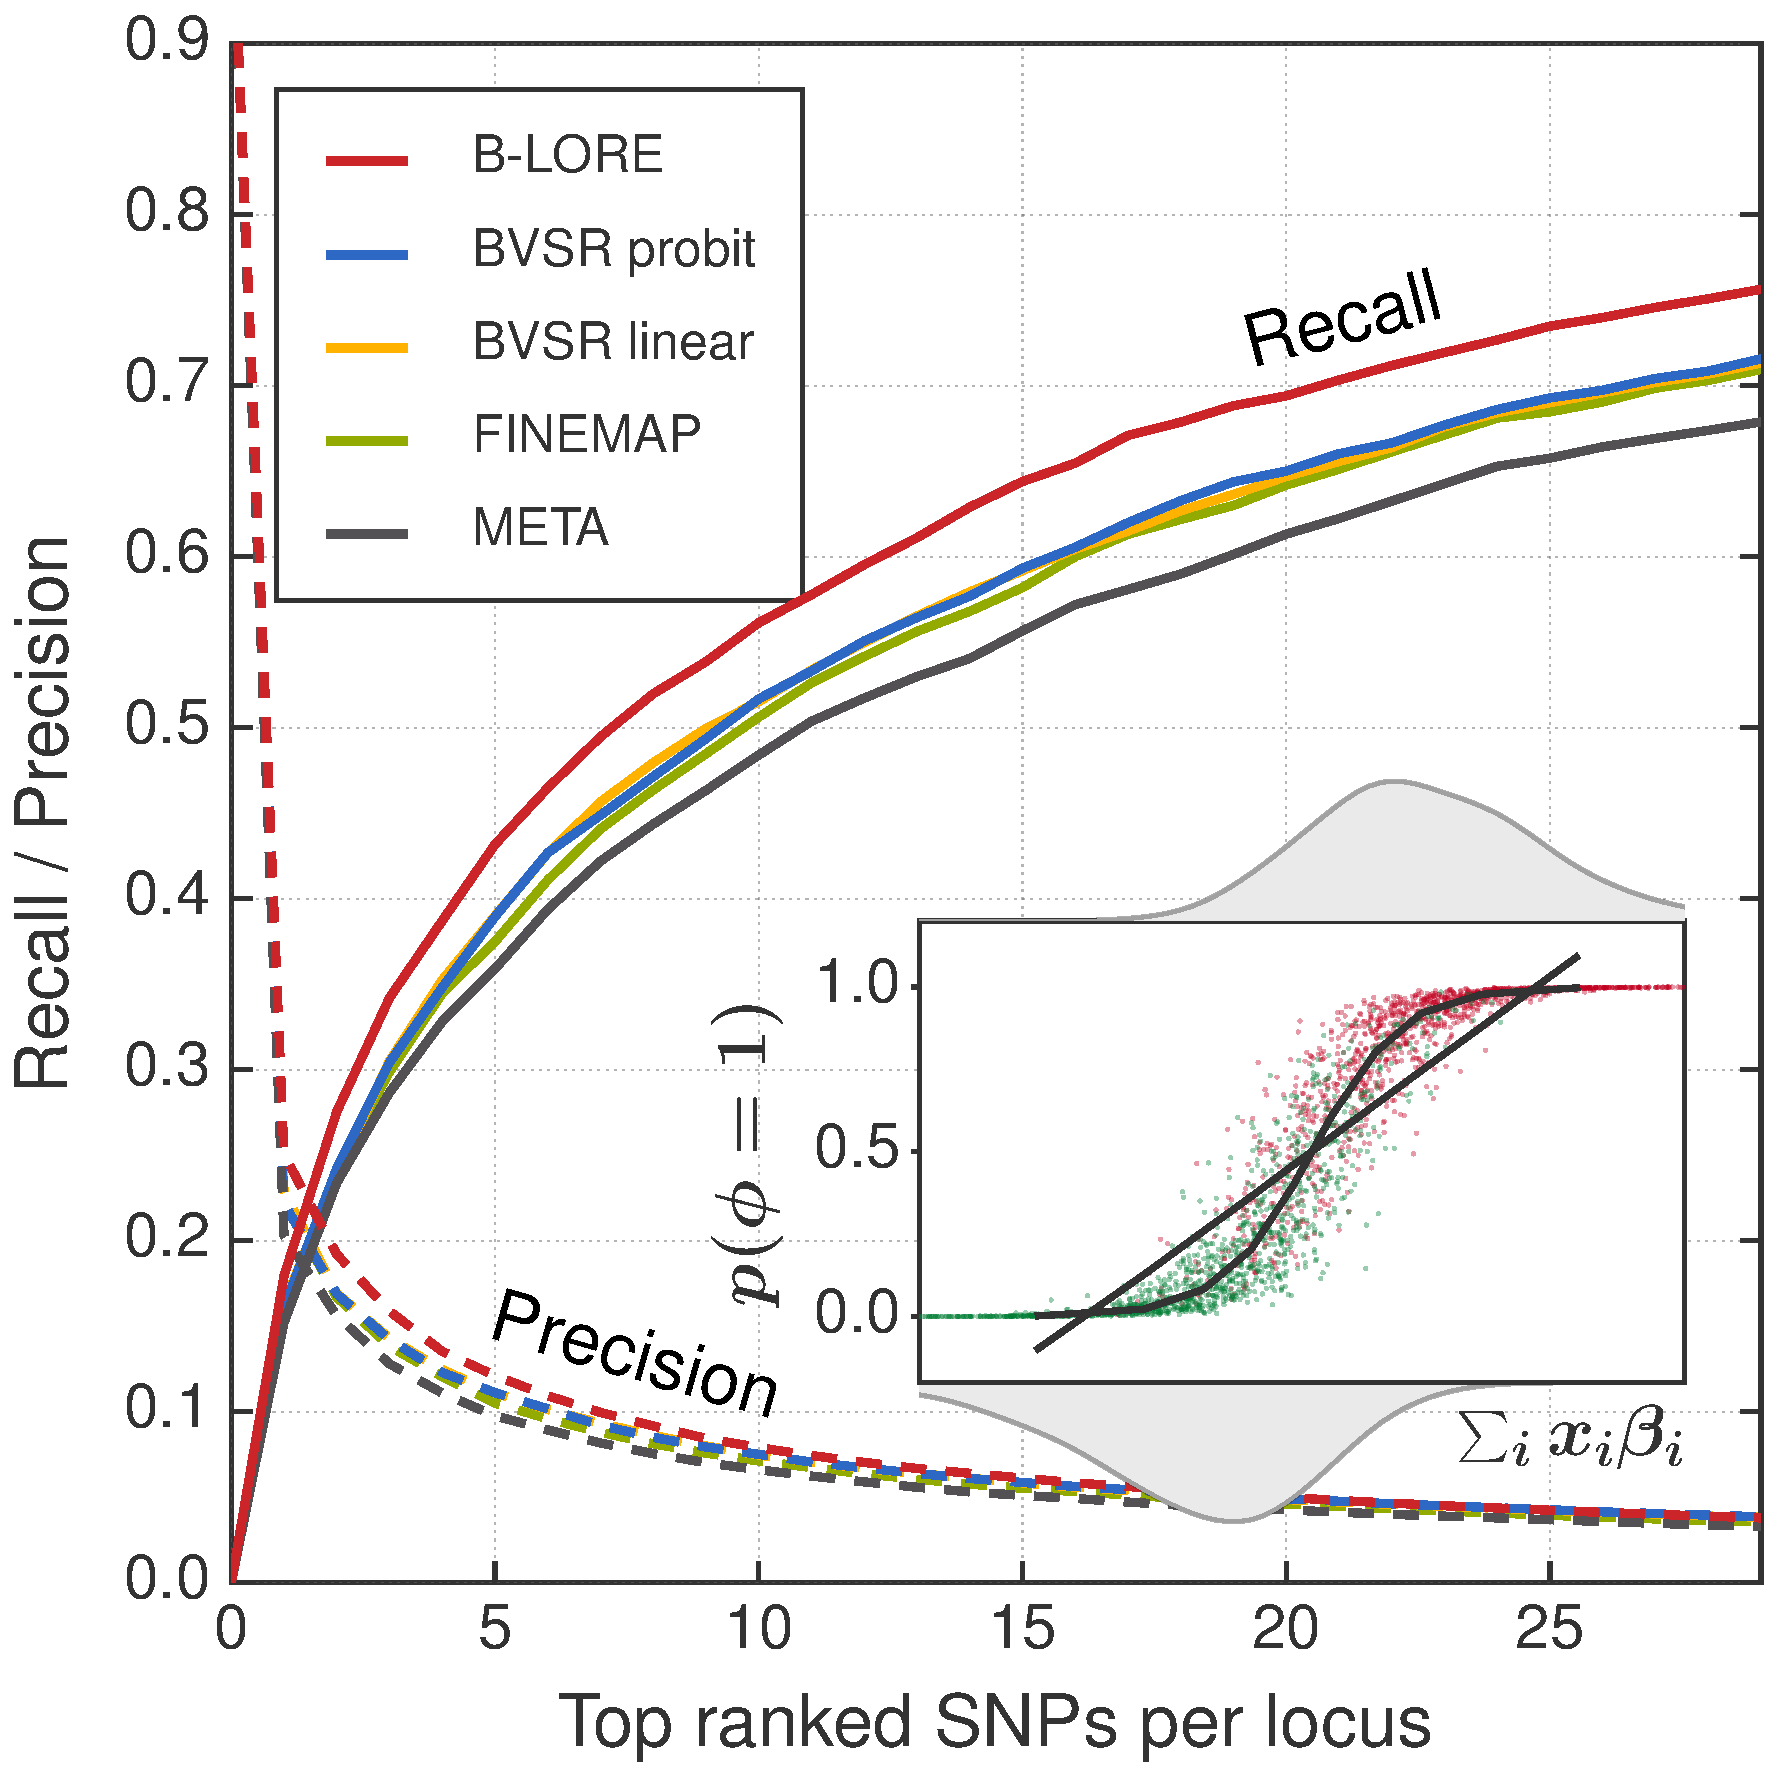
\includegraphics[width=0.23\textwidth]{pip_prc_normal_h08_c2_l100_cred.pdf}
   \end{center}
  }
  {\begin{center}
   Case/Control = 1.0 \\
   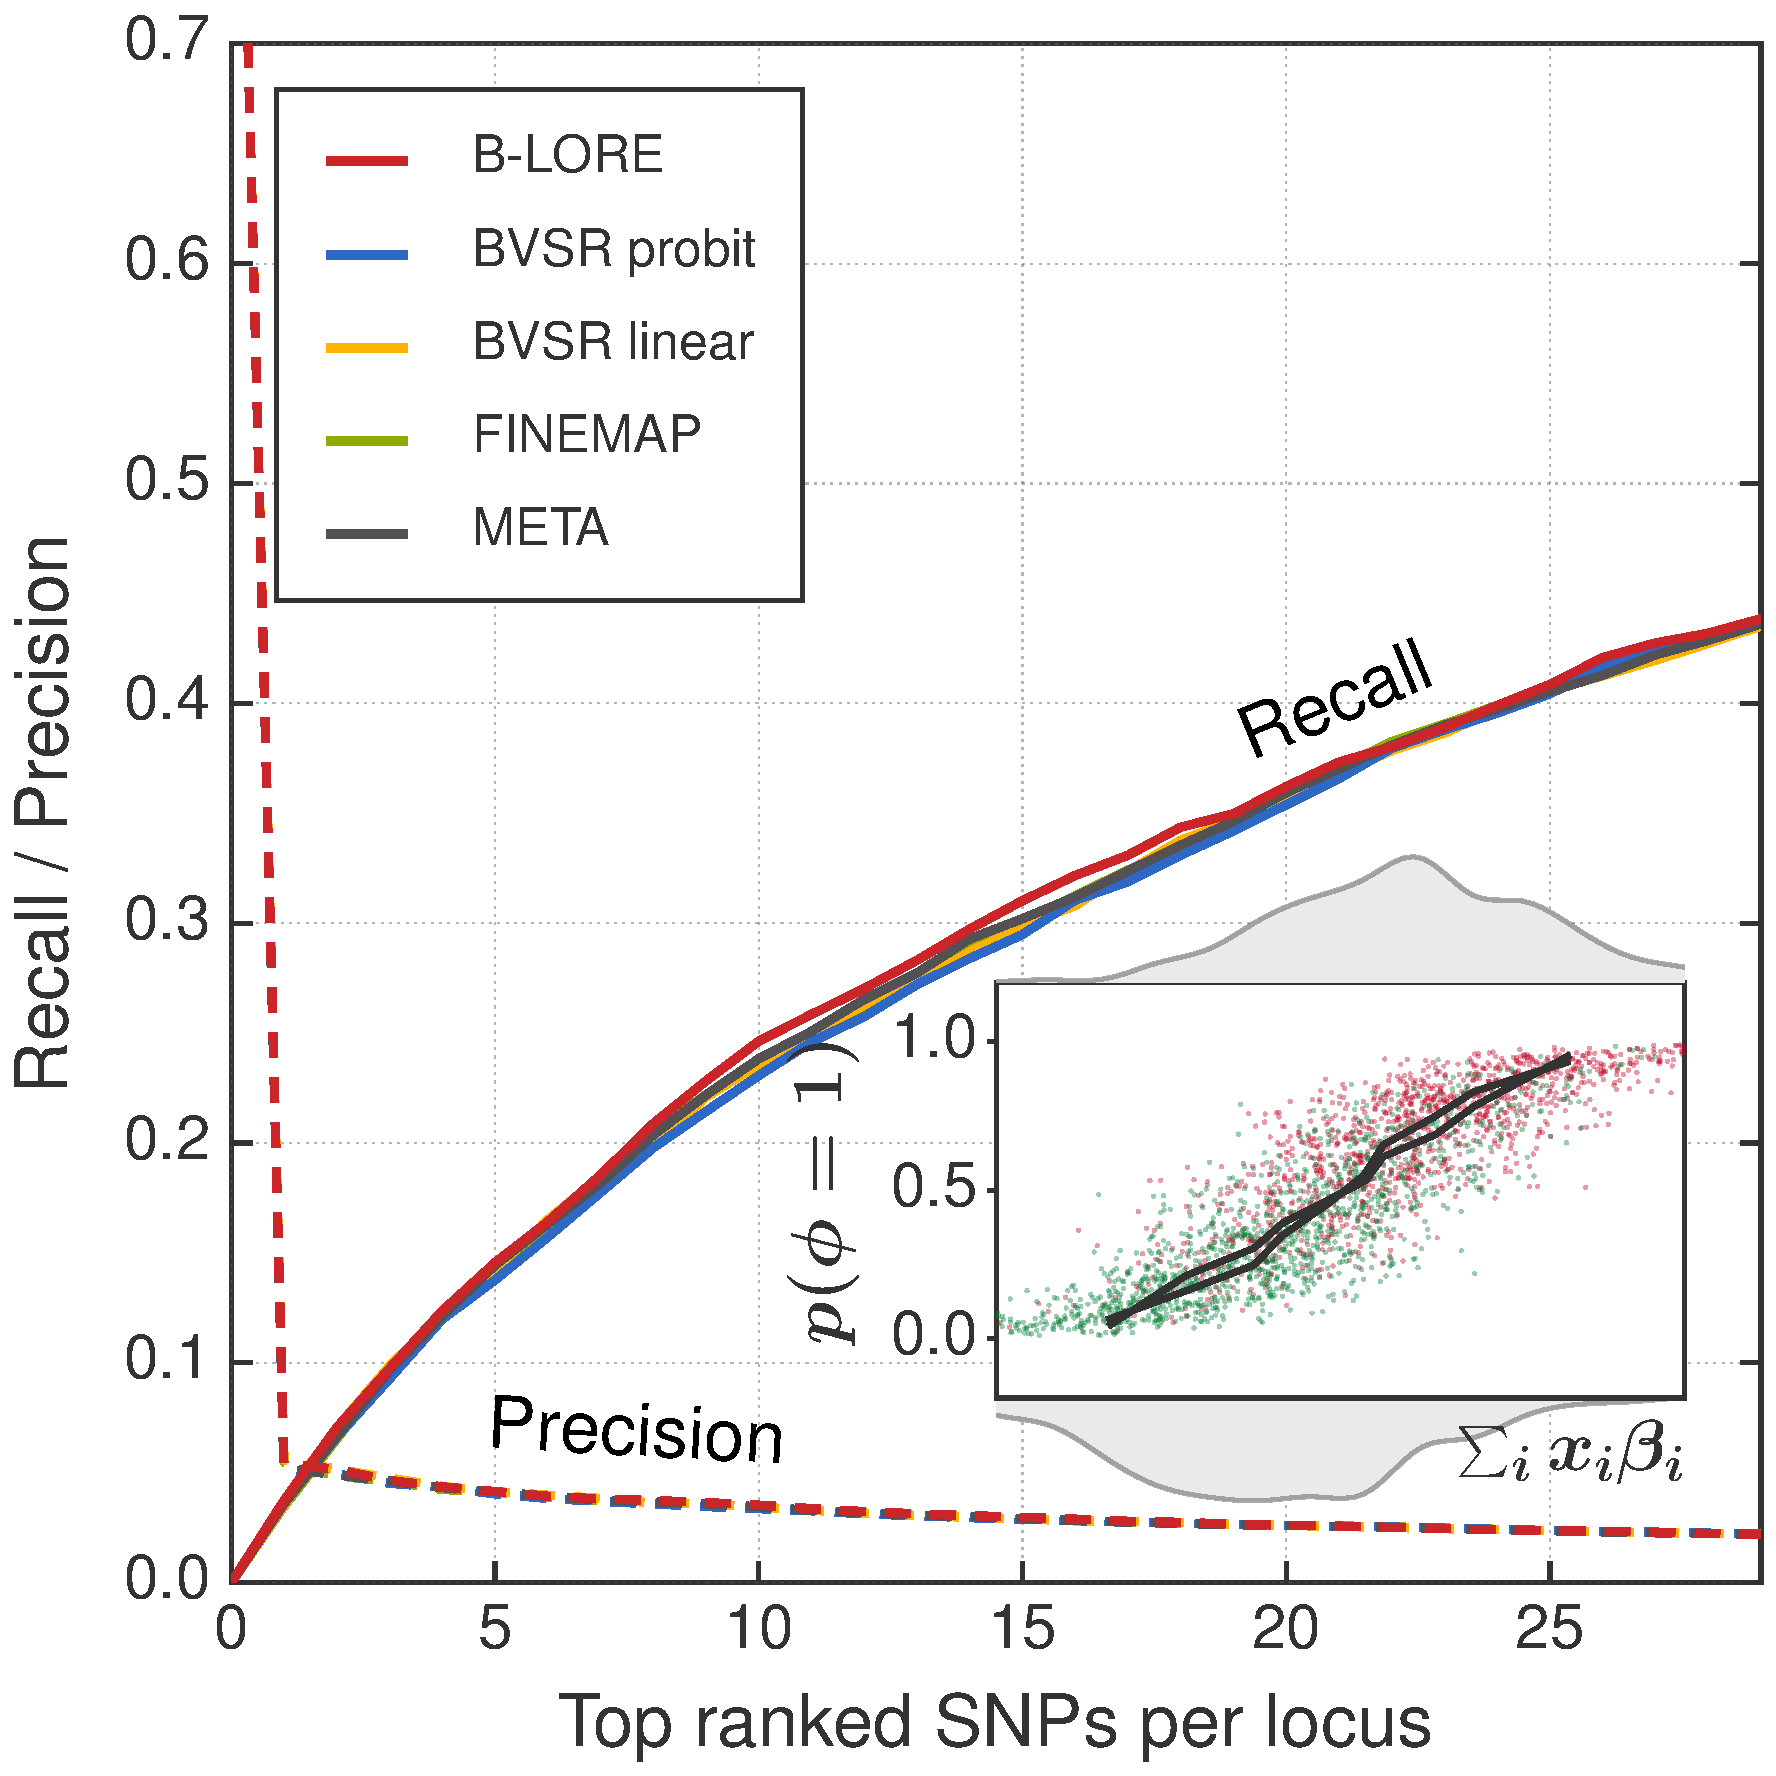
\includegraphics[width=0.23\textwidth]{pip_prc_normal_h04_c2_l100_fixcase_cred.pdf}
   \end{center}
  }
  {\begin{center}
   Case/Control = 0.25 \\
   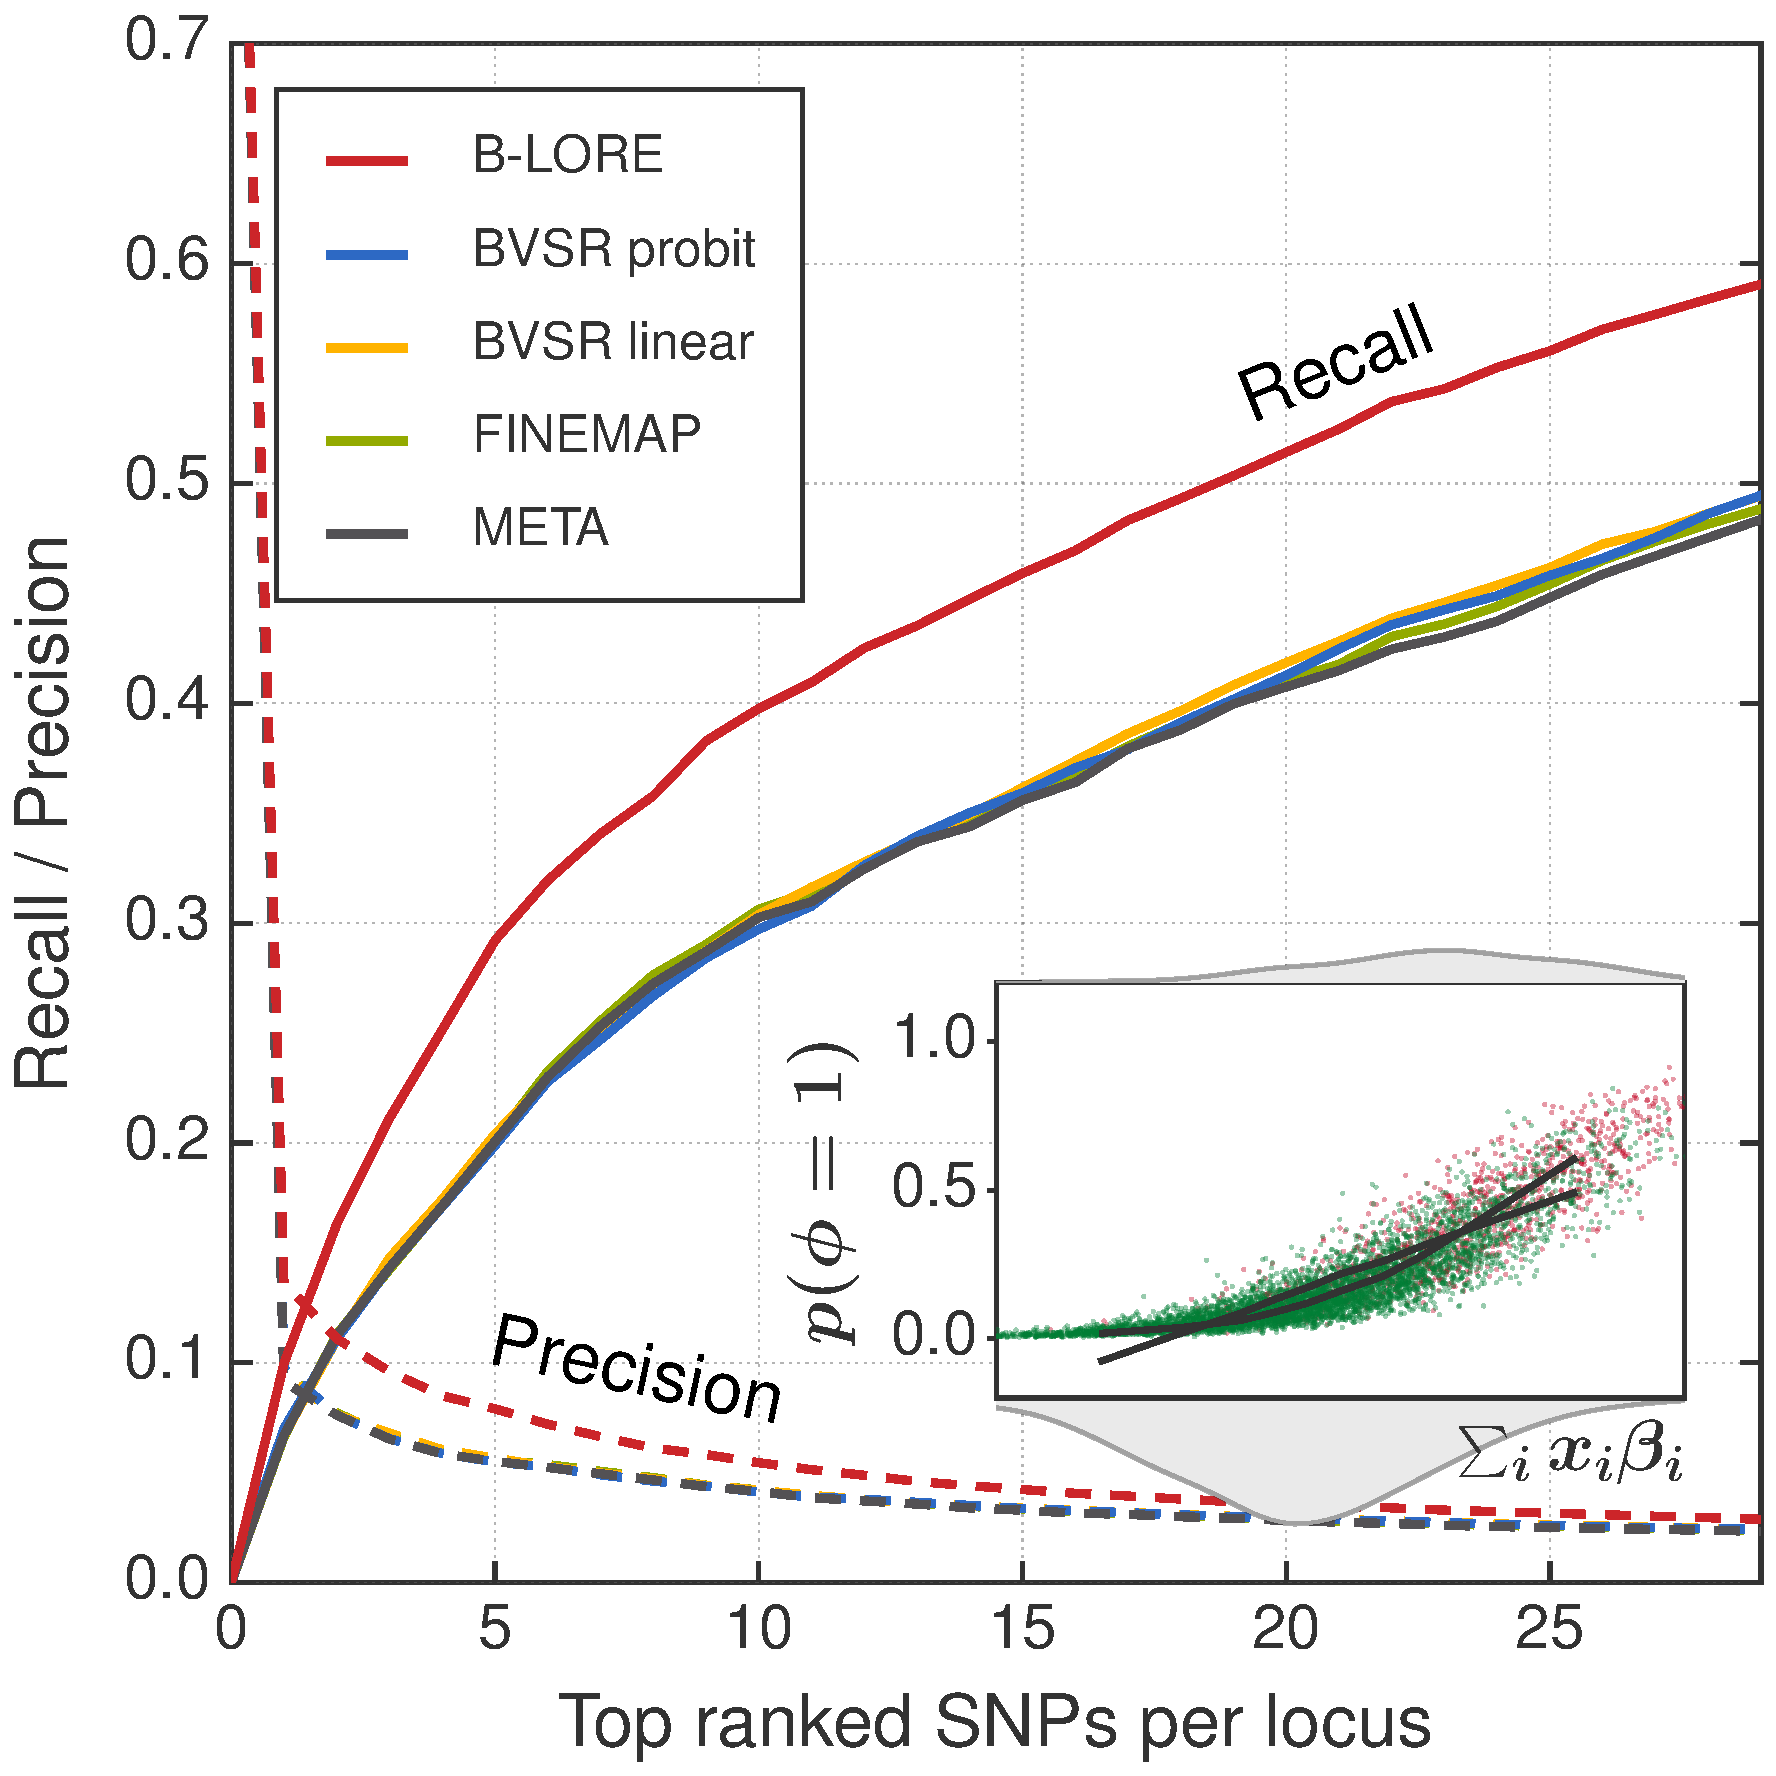
\includegraphics[width=0.23\textwidth]{pip_prc_normal_h04_c2_l025_fixcase_cred.pdf}
   \end{center}
  }
\end{multicols}
}

%%%%%%%%%%%%%%%%%%%%%%%%%%%%%%%%%%
%%%% REFERENCES %%%
%%%%%%%%%%%%%%%%%%%%%%%%%%%%%%%%%%
\headerbox{7. References}{name=biblio, column=3, span=1, below=realcad, below=infer}{
 {\raggedright
  \footnotesize
 \begin{enumerate}[leftmargin=1.5em]
   \item Banerjee \etal PLOS Genet 2018, doi:10.1371/journal.pgen.1007856
   \item Servin \etal PLOS Genet 2007, doi:10.1371/ journal.pgen.0030114
   \item Guan \etal Ann Appl Stat 2011, doi:10.1214/ 11-AOAS455
   \item CARDIoGRAMplusC4D Nat Genet 2015, doi:10.1038/ng.3396
 \end{enumerate}
 }
}

\headerbox{8. Acknowledgement}{name=thanks, column=3, span=1, below=biblio}{

  \footnotesize
  We thank Prof. Dr. Jeanette Erdmann for helpful discussions.
  This work was supported by the German Federal Ministry of Education and Research (BMBF) within the framework of
  the e:Med research and funding concept (grant 01ZX1313A-2014).

  %\begin{multicols}{2}
  %  
\includegraphics[height=55px]{BMBF.eps}
  %  
\includegraphics[height=27px]{emed_logo.png}
  %\end{multicols}

  %%\vskip-0.5em
  \colorbox{light} {
  \begin{minipage}{0.95\textwidth}
    \centering
    \raisebox{-0.5\height}{
\includegraphics[height=57px]{BMBF.eps}}
    %\hspace*{.2in}
    \raisebox{-0.5\height}{
\includegraphics[height=27px]{emed_logo.png}}
  \end{minipage} } \par
}



%%%%%%%%%%%%%%%%%%%%%%%%%%%%%%%%%%%
%%%% ACKNOWLEDGEMETS %%%
%%%%%%%%%%%%%%%%%%%%%%%%%%%%%%%%%%%
%\headerbox{5 Case Study: Helix-Helix Contacts in  YidC }{name=yidc, column=1, row=1, span=1, below=cc}{
%	
%	
%	\begin{multicols}{2}	
%	
%	\includegraphics[height=150px]{YidC_couplingmatrix}
%	Statistical residue-residue coupling analysis was applied to the bacterial transmembrane protein YidC. 
%	We then computed probabilities for each possible helix-helix contact by aggregating the evidence of stronger coupling coefficients over the expected interaction patterns. 
%	A structural model built from this co-evolutionary analysis was found to be consistent with recently published crystal structures of YidC (Kumazaki et al, Nature 2014). 
%	\end{multicols}
%	
%	\vspace{-1.5em}
%	\centering
%	\includegraphics[height=115px]{YidC_model}
%	
%}
%
%
%%%%%%%%%%%%%%%%%%%%%%%%%%%%%%%%%%%
%%%% 6 Predicting Distance Maps %%%
%%%%%%%%%%%%%%%%%%%%%%%%%%%%%%%%%%%
%
%\headerbox{6 Predicting Inter-residue Distances}{name=distancemaps, column=1, row=2, span=1, below=yidc,above=bottom}{
%	
%The definition of residue contacts is based on a rigid distance threshold, e.g. $C_{\beta}$-8\si{\angstrom}. Since residue interactions span much broader distance ranges, it is biologically meaningful to extend the concept of binary contacts. Using statistical modeling we aim at predicting inter-residue distances. The resulting increased information content of distance maps has already been shown to boost precision of predicted structural models (Kukic et al.,(2014)).
%
%	\includegraphics[height=125px]{residue_distance_profile}
%	\includegraphics[height=125px]{distance_map}
%	
%%	\includegraphics[height=110px]{residue_distance_structure}
%
%}
%

\end{poster}
\end{document}
